\documentclass[dvipdfmx, a4paper, 9pt]{deimj}

\usepackage[T1]{fontenc}
\usepackage{lmodern}
\usepackage{graphicx}
\usepackage{url}
\usepackage{bmpsize}

% TikZ関連パッケージ
\usepackage{tikz}
\usetikzlibrary{shapes.geometric, arrows.meta, positioning, calc, fit, backgrounds}

% 追加パッケージ
\usepackage{amsmath, amssymb}
\usepackage{bm}
\usepackage{booktabs}
\usepackage{array}
\usepackage{tabularx}

% 印刷位置調整
\hoffset -10mm
\voffset -10mm

\newcommand{\AmSLaTeX}{%
 $\mathcal A$\lower.4ex\hbox{$\!\mathcal M\!$}$\mathcal S$-\LaTeX}
\newcommand{\PS}{{\scshape Post\-Script}}
\def\BibTeX{{\rmfamily B\kern-.05em{\scshape i\kern-.025em b}\kern-.08em
 T\kern-.1667em\lower.7ex\hbox{E}\kern-.125em X}}

% TikZ用設定
\tikzset{
    base/.style={rectangle, draw, rounded corners, inner sep=5pt, align=center, font=\scriptsize, fill=white, line width=0.6pt},
    llm/.style={base, fill=blue!5, draw=blue!70!black},
    storage/.style={base, fill=orange!5, draw=orange!70!black},
    mcp/.style={base, fill=purple!5, draw=purple!70!black},
    blender/.style={base, fill=green!5, draw=green!70!black},
    client/.style={base, fill=blue!5, draw=blue!70!black},
    tools/.style={base, fill=purple!2, draw=purple!50!black},
    blender_proc/.style={base, fill=green!5, draw=green!70!black},
    addon/.style={base, fill=green!2, draw=green!50!black},
    group/.style={draw, dashed, inner sep=5pt, rounded corners, fill=gray!5},
    subgroup/.style={draw, solid, inner sep=4pt, rounded corners, fill=white, line width=0.6pt},
    group_label/.style={font=\sffamily\bfseries\scriptsize},
    arrow/.style={-{Stealth[inset=1.5pt, length=5pt, width=4pt]}, line width=0.5pt, draw=black!80},
    darrow/.style={{Stealth[inset=1.5pt, length=5pt, width=4pt]}-{Stealth[inset=1.5pt, length=5pt, width=4pt]}, line width=0.5pt, draw=black!80},
    dashed_arrow/.style={-{Stealth[inset=1.5pt, length=5pt, width=4pt]}, dashed, line width=0.5pt, draw=black!80}
}

\newcommand{\tightlabel}[1]{{\xkanjiskip=0pt #1}}

% タイトル設定
\jtitle{Model Context Protocolを用いた二層知識継承による\\建築制約を持つ屋内シーン生成の自律的品質保証}

% 著者リスト
\authorlist{%
 \authorentry[s2422110@stu.musashino-u.ac.jp]{多田 有里}{Yuri Tada}{MU}%
 \authorentry[ryonaka@musashino-u.ac.jp]{中村 亮太}{Ryota Nakamura}{MU}%
}

% 所属設定
\affiliate[MU]{武蔵野大学データサイエンス学部\hskip1zw
  〒135--8181 東京都江東区有明3丁目3--3}
 {Faculty of Data Science, Musashino University,
  3-3-3 Ariake, Koto-ku, Tokyo 135--8181, Japan}

\begin{document}
\pagestyle{empty}

% 和文あらまし
\begin{jabstract}
近年の生成AIの進展により，Text-to-3D技術は飛躍的な視覚的品質を達成したが，既存手法はレンダリング画像の「自然さ」を優先するため，物理的・工学的整合性を欠く問題（本稿では幾何学的ハルシネーションと定義する）が未解決の課題となっている．本研究では，幾何学的ハルシネーションという課題に対し，Model Context Protocol (MCP) を基盤とした自律的品質保証フレームワークを提案する．提案手法は，LLMと3D環境（Blender）を接続し，視覚情報ではなく数値データ（座標，法線，寸法）に基づいてモデルを直接検査・修正する「生成・検査・修正」サイクルを自律的に実行する．

システムは，不変の「規制知識」と適応的な「経験知識」からなる二層知識構造を有し，過去の修正プロセスから効率的な方策を獲得する知識継承メカニズムを備えている．建築制約を持つ生成タスクにおける評価実験の結果，提案手法は視覚ベースでは困難な厳密な制約充足を達成した．さらに，性能推移の分析により，知識の蓄積が自律性スコアを最大値の「5」まで向上させ，初期試行と比較してトークン消費量を約58\%削減することを定量的に実証した．提案するアプローチは，3D生成の評価軸を主観的な「見た目」から客観的な「構造的整合性」へと拡張し，エンジニアリングツールとしての生成AIの可能性を拓くものである．
\end{jabstract}

% キーワード
\begin{jkeyword}
Text-to-3D，Model Context Protocol，Generative AI，Quality Assurance，Knowledge Inheritance
\end{jkeyword}

\maketitle

%%%%%%%%%%%%%%%%%%%%%%%%%%%%%%%%%%%%%%%%%%%%%%%%%%%%%%%%%%%%%%%%%%%%%%%
\section{はじめに}
%%%%%%%%%%%%%%%%%%%%%%%%%%%%%%%%%%%%%%%%%%%%%%%%%%%%%%%%%%%%%%%%%%%%%%%

\subsection{研究の背景：視覚的「自然さ」から構造的「整合性」へ}

近年，生成AI技術の進展は目覚ましく，テキストから画像，映像，そして3Dモデルを生成することが日常的な技術となりつつある．特に大規模言語モデル（LLM）を用いた「3D-GPT」\cite{sun20233dgpt}のようなプロシージャル生成フレームワークは，専門的なスキルを持たないユーザでも複雑な3Dシーンを構築できる可能性を切り開いた．しかし，既存のText-to-3D技術が生み出す成果物は，レンダリング画像としての視覚的な「自然さ」において優れている一方で，構造的な「整合性」や物理的な「妥当性」において致命的な欠陥を抱えることが多い．

本稿では，**幾何学的ハルシネーション（geometric hallucination）**とは，レンダリング画像上は自然に見えるにもかかわらず，3D空間内の幾何・物理・法規的制約（例：接地，干渉回避，包含，寸法整合，法規に基づく数値条件）を満たさない状態を指すと定義する．本研究では特に，視覚的評価指標（例：画像特徴に基づく類似度）だけでは検出が難しい「構造的違反」を対象とし，以下のカテゴリに整理する．
\begin{enumerate}
    \item[(i)] \textbf{接地性違反}：床面への支持がなく浮遊している．
    \item[(ii)] \textbf{干渉（衝突）違反}：オブジェクト同士が体積的に重なっている．
    \item[(iii)] \textbf{包含・埋没違反}：壁や床に不適切に埋まる／外部へ突き抜ける．
    \item[(iv)] \textbf{寸法・整列違反}：垂直・水平，段差，クリアランス等が不整合．
    \item[(v)] \textbf{法規・設計数値違反}：採光面積等，数値として定義可能な設計条件を満たさない．
\end{enumerate}
以上を「幾何学的ハルシネーション」として包括し，以降では各カテゴリを数値判定可能な制約として実装する．

幾何学的ハルシネーションが生じる根源は，現在の生成パラダイムがCLIPスコア\cite{radford2021clip}やLPIPS\cite{zhang2018lpips}といった「視覚的評価」に過度に依存している点にある．VLMは画像の類似性を判断できても，「垂直性」「接地性」「包含関係」といった3D空間特有の厳密な幾何学的制約を，2D画像から正確に逆推論することは本質的に困難である．

\subsection{研究の目的}

本研究の目的は，建築制約を持つ屋内3Dシーン生成において，視覚情報に依存せず，数値データに基づく厳密な検査のみを用いた自律的品質保証フレームワークを構築することである．特に，静的な法規制を格納するStaticDBと，動的な経験知識を蓄積するDynamicDBを分離・統合するアーキテクチャにより，幾何学的整合性の保証と，試行回数の削減による推論コストの最適化を同時に達成することを，定量的に実証する．

\subsection{解決へのアプローチ：MCPによる数値的介入と知識の永続化}

人間は視覚情報のみから，物体の安定性や支持関係の破綻（例：浮遊，倒れそうな配置）を一定程度推定できることが知られている．また仮想環境における“もっともらしさ（plausibility）”の破れは，空間的没入感や体験品質に影響しうる．しかし，こうした人間の主観評価は暗黙的・文脈依存であり，設計要件として再利用可能な形で明示されにくい．そこで本研究では，違和感の原因となりやすい支持・干渉・包含・寸法整合といった構造条件を，3D空間上の数値制約として形式化し，決定論的に検査可能な品質保証へ接続する．

具体的には，Model Context Protocol (MCP)\cite{anthropic2024mcp} を介してLLMを3Dモデリング環境（Blender）に直接接続し，エージェントが3D空間を座標や寸法といった「数値データ」として認識・操作するアーキテクチャを構築する．

提案システムの特徴は，書き換え不可能な規制知識を扱うStaticDBと，ユーザからのフィードバックを通じて成長する経験知識を扱うDynamicDBを分離した二層知識モデルにある．エージェントは，物理法則や建築基準法といった絶対的なルールを遵守しつつ，対話を通じて得た修正指示を新たなルールとして知識ベースに蓄積する．知識の永続化により，セッションごとに記憶がリセットされる従来のLLMエージェントの限界を克服し，使い込むほどに文脈理解が深化し，推論コストが最適化される「経験を蓄積するパートナー」としてのAIを実現する．

\subsection{提案手法の貢献}

本研究の主な貢献は以下の2点に集約される．本質的に，提案手法はText-to-3Dという特定のドメインに留まらず，「数値的に検証可能な生成タスク一般」に対して適用可能な，普遍的な品質保証原理を示唆している．
\begin{enumerate}
    \item \textbf{数値検査に基づくMCPループの構築:} 
    視覚的評価を完全に排除し，MCPを介して3D座標・法線データを直接検証するループを実装した点．数値的な検証により，画像ベースの手法では検出不可能なオクルージョン領域や微細な位置ズレの修正を可能にした．
    \item \textbf{二層知識構造による探索の効率化:} 
    エージェントの知識を不変の「規制」と可変の「戦略」に分離し，修正プロセスで得た成功パターンを永続化するメカニズムを実装した点．経験の蓄積により，初期のランダムな探索から，知識検索による即時解決へと行動を変容させることが可能となった．
\end{enumerate}

%%%%%%%%%%%%%%%%%%%%%%%%%%%%%%%%%%%%%%%%%%%%%%%%%%%%%%%%%%%%%%%%%%%%%%%
\section{関連研究}
%%%%%%%%%%%%%%%%%%%%%%%%%%%%%%%%%%%%%%%%%%%%%%%%%%%%%%%%%%%%%%%%%%%%%%%

第2章では，Text-to-3D技術における評価指標の変遷と課題，およびLLMを用いた3D操作に関する近年の研究動向を概観する．特に，既存の視覚ベースのフィードバックループが抱える限界を指摘し，提案するアプローチが採用するMCPを用いた構造的検証アプローチの優位性と学術的位置付けを明確にする．

\subsection{3D生成モデルにおける評価指標の変遷と課題}

3Dコンピュータビジョンとグラフィックスの分野は，深層学習の導入により劇的な変革を遂げている．初期の3D生成モデルは，点群やボクセル，メッシュといった明示的な3D表現を直接生成することを目的としており，初期の3D生成モデルの評価にはChamfer Distance (CD) やEarth Mover's Distance (EMD) といった幾何学的距離指標が標準的に用いられてきた\cite{fan2017point,nichol2022point}．幾何学的距離指標は，生成された形状と正解データとの間の物理的な距離を測定するため，幾何学的な忠実度を保証する上では一定の有効性を持つ．しかし，CDは点密度の不均一性に鈍感である「不感領域」の問題を抱え，EMDは計算コストが非常に高いという実用上の課題があった．

その後，Neural Radiance Fields (NeRF)\cite{mildenhall2020nerf} や3D Gaussian Splatting (3DGS)\cite{kerbl20233dgs} の登場により，パラダイムは「画像からの逆投影」による生成へとシフトした．生成パラダイムのシフトに伴い，評価指標もPSNR，SSIM，そしてLPIPS\cite{zhang2018lpips}やCLIP Score\cite{radford2021clip}といった画像空間での知覚的類似性指標が主流となった．特にLPIPSは人間の知覚と高い相関を持つとされるが，画像空間での知覚的類似性指標は本質的に「2Dの見た目」を評価するものであり，3D構造としての整合性を保証しない．

例えば，ある視点からは整合して見えるが，裏側が欠損している，あるいは物体同士が物理的に不可能な交差をしているといった問題（2Dチーティング）は，画像ベースの指標では検出困難である\cite{poole2022dreamfusion}．建築やプロダクトデザインのようなエンジニアリンググレードの整合性が求められる領域において，画像空間での指標のみを追求する指標は不十分であり，構造的な「妥当性」を担保する新たな枠組みが必要とされている．

\subsection{LLMによる3D空間操作と視覚フィードバックの限界}

LLMの高い推論能力を活かし，エージェントとして3D空間を操作させる試みも始まっている．代表的な研究であるSceneCraft\cite{hu2024scenecraft}は，ユーザの自然言語指示をBlenderのPythonスクリプトに変換し，Pythonスクリプトの実行結果をレンダリング画像として取得，マルチモーダルLLM (MLLM) で解析することで修正ループを回す手法を提案した．SceneCraftによるアプローチは，プログラマティックな操作により幾何学的構造をある程度制御できる点で画期的である．

しかし，SceneCraft等の既存手法は「視覚フィードバック」に依存しているため，VLMの空間認識能力の限界に縛られるという課題がある．視覚情報は3次元情報の2次元への圧縮（射影）であり，そこから完全な3D構造を復元・評価することは逆問題として本質的な不安定さを孕んでいる．例えば，「物体が床から数ミリ浮いている」といった微細な誤差や，「壁の内部に配管が正しく通っているか」といったオクルージョンの検証は，2D画像からは原理的に不可能に近い．

したがって，正確な3Dモデリングを実現するためには，視覚情報に頼らない，シーンデータ（頂点座標，法線ベクトル，バウンディングボックス等）への直接的なアクセスと，数値に基づく論理的な検証が必要となる．

\subsection{MCPとエージェントの自律性}

Anthropicによって導入されたMCP\cite{anthropic2024mcp} は，AIモデルと外部ツール間の通信を標準化するオープンプロトコルであり，エージェントシステムの実装に革新をもたらしている．従来の関数呼び出しが単発の関数実行を目的としていたのに対し\cite{schick2024toolformer}，MCPはクライアント・サーバ間のステートフルな接続を維持し，リソースの購読やプロンプトのテンプレート化，そして何より「Sampling」プリミティブによる双方向のインタラクションをサポートしている点がMCPの特徴である．

「Sampling」機能は，サーバ側（ツール側）からクライアント（LLM）に対して，コンテキストを与えた上で次の行動を能動的に問い合わせることを可能にする．Sampling機能により，エージェントは自身の行動結果（ツールの出力やエラーメッセージ）を受け取り，行動結果を評価して次の行動を決定する自律的なループ（ReActサイクル\cite{yao2023react}や自己修正ループ\cite{shinn2024reflexion,xi2023rise}）を，標準化されたプロトコル上で堅牢に実装可能となる．

既存のUnrealMCP\cite{unrealmcp2024}などの実装は，自然言語によるコマンド実行を可能にしたが，体系的な評価フレームワークや，失敗から学ぶ自己改善ループまでは実装されていないのが現状である．

既存研究には，LLMによる3D生成・編集や，視覚フィードバックを用いた反復的改善の枠組みが提案されている．一方で，(a) 数値制約に基づく体系的な検査（quality checking），(b) 検査結果に基づく自動修正の反復（self-correction loop），\textbf{(c) セッションを跨いで知識を永続化し効率を改善する仕組み（knowledge inheritance）}を，統合的に扱う研究は依然として限定的である．本研究はこの統合に焦点を当て，幾何・法規に由来する数値制約を扱う品質保証ループと，二層知識ベースによる継承メカニズムを提案する．

\subsection{本研究の位置付けと新規性の要約}

前述した既存手法と本提案手法の主要な差分を表\ref{tab:comparison}にまとめる．本研究の核心的な新規性は，視覚情報の曖昧さを排除した「数値ベースのMCPループ」と，セッションを跨いで戦略を継承する「二層知識構造」を統合した点にある．

\begin{table}[ht]
  \caption{既存の3D生成フィードバック手法と本提案手法の比較}
  \label{tab:comparison}
  \centering
  % \hspace{-5mm}
  \small
  \begin{tabularx}{\columnwidth}{lXX}
    \toprule
    比較項目 & 既存手法（SceneCraft等） & 提案手法（Dual-Knowledge MCP）\\
    \midrule
    評価の根拠 & 2Dレンダリング画像（視覚） & 3D座標・寸法（数値）\\
    検証の対象 & 知覚的なもっともらしさ & 幾何学的・法規的な整合性\\
    通信方式 & 単発のスクリプト実行 & MCPによる双方向・状態保持通信\\
    エラー検知 & VLMによる画像解析 & 幾何計算による決定論的判定\\
    知識の扱い & セッションごとにリセット & 二層構造（Static/Dynamic）で永続化\\
    \bottomrule
  \end{tabularx}
\end{table}

%%%%%%%%%%%%%%%%%%%%%%%%%%%%%%%%%%%%%%%%%%%%%%%%%%%%%%%%%%%%%%%%%%%%%%%
\section{提案手法}
%%%%%%%%%%%%%%%%%%%%%%%%%%%%%%%%%%%%%%%%%%%%%%%%%%%%%%%%%%%%%%%%%%%%%%%

第3章では，3Dモデリングにおける構造的な整合性の担保と，経験に基づく適応的な戦略獲得を実現するためのシステムアーキテクチャ「Dual-Knowledge MCP Architecture」について詳述する．提案した構成の中核は，推論能力と実行環境を標準プロトコルで疎結合に接続し，静的な規制知識と動的な経験知識という性質の異なる二つの知識源を統合的に運用する点にある．

\subsection{システムアーキテクチャの全体構想}

提案システムの設計思想は，高度な推論を行うAIコア（LLM）と，物理的なシミュレーションを行う3D環境（Blender\cite{community2018blender}）を明確に分離し，AIコアと3D環境の間を標準化されたインターフェース（MCP）で調停することにある．MCPを用いた疎結合な設計により，特定のLLMや3Dソフトウェアに依存しない拡張性と，各コンポーネントの独立した進化を担保している．

システムの全体的な概念図を図\ref{fig:architecture}に示す．アーキテクチャは主に4つの論理階層によって構成される．

\begin{figure}[t]
  \centering
  \resizebox{0.95\columnwidth}{!}{%
  \begin{tikzpicture}[scale=1.1, every node/.style={scale=1.0}]
      \coordinate (Origin) at (0,0);
      % ノードの定義
      \node (User) [base] at ($(Origin) + (-1.5, 2.0)$) {ユーザ};
      \node (Input) [base] at ($(Origin) + (-1.5,  1.3)$) {自然言語プロンプト};
      \node (LLM) [llm] at ($(Origin) + (-1.5, 0.1)$) {\tightlabel{\mbox{ローカルLLM}}};
      \node (Planner)  [llm]  at ($(Origin) + (-1.5, -0.9)$) {プランナー\\モジュール};
      \node (StaticDB)  [storage] at ($(Origin) + (2.0,  -0.35)$) {StaticDB};
      \node (DynamicDB) [storage] at ($(Origin) + (2.0, -1.05)$) {DynamicDB};
      \node (Router) [mcp] at ($(Origin) + (-1.5, -2.1)$) {\tightlabel{\mbox{MCPルーター}}};
      \node (T1) [mcp] at ($(Origin) + (-2.2, -3.2)$) {T1: 操作};
      \node (T2) [mcp] at ($(Origin) + (-0.8, -3.2)$) {T2: 空間};
      \node (T3) [mcp] at ($(Origin) + ( 0.6, -3.2)$) {T3: 検査};
      \node (T4) [mcp] at ($(Origin) + ( 2.0, -3.2)$) {T4: 知識};
      \node (API)   [blender] at ($(Origin) + (-1.5, -4.7)$) {Python API\\(bpy)};
      \node (Scene) [blender] at ($(Origin) + ( 1.5, -4.7)$) {3Dシーン\\状態};
      \node (BlenderEnv) [blender] at ($(Origin) + (1.5, -5.7)$) {ビューポート(GUI)};
      % グループ化
      \begin{scope}[on background layer]
          \node (User_Layer) [group, fit=(User) (Input), label={[group_label]north:\tightlabel{ユーザ層}}] {};
          \node (AI_Core)    [group, fit=(LLM) (Planner), label={[group_label, xshift=-0.7cm,yshift=-0.1cm]north:\tightlabel{\mbox{AIコア層}}}] {};
          \node (KB)         [group, fit=(StaticDB) (DynamicDB), label={[group_label]north:\tightlabel{知識層}}] {};
          \node (Tools)      [group, fit=(T1) (T4)] {};
          \node (MCP_Layer)  [group, fit=(Router) (Tools), label={[group_label]south:\tightlabel{\mbox{MCP統合層}}}] {};
          \node (Exec)       [group, fit=(API) (Scene) (BlenderEnv), label={[group_label]below:\tightlabel{\mbox{Blender環境層}}}] {};
      \end{scope}

      % 接続
      \draw [arrow] (User) -- (Input);
      \draw [arrow] (Input) -- (LLM);
      \draw [darrow] (LLM) -- (Planner);
      \draw [arrow] (Planner) -- (Router);
      \foreach \t in {T1, T2, T3, T4} {
          \draw [arrow] (Router.south) -- ++(0,-0.2) -|
          (\t.north);
      }
      \draw [arrow] (StaticDB.west) -| ([xshift=0.2cm]T3.north);
      \draw [arrow] (Scene.north) -- (T3.south);
      \draw [darrow] ([xshift=0.2cm]DynamicDB.south) -- ([xshift=0.2cm]T4.north);
      \draw [dashed_arrow] ([xshift=-0.2cm]T4.north) --  ([xshift=0.5cm]Planner.south);
      \draw [arrow] (T1.south) -- ([xshift=-0.2cm]API.north);
      \draw [arrow] (T2.south) -- ([xshift=0.2cm]API.north);
      \draw [darrow] (API) -- (Scene);
      \draw [arrow] (Scene) -- (BlenderEnv);
      % フィードバックループの矢印を破線に変更
      \draw [dashed_arrow] ([xshift=-2mm]T3.north) |- (0,0.1) -- (LLM.0);
  \end{tikzpicture}%
  }
  \caption{提案システムの概念的アーキテクチャ図（図中の破線はフィードバックおよび知識参照を示す）}
  \label{fig:architecture}
\end{figure}

\subsubsection{AIコア層：推論と計画}

本システムの中心モジュールは，(i) 目的の分解と手順の構築を行う推論・計画モジュール，(ii) ツール実行結果（数値ログ）を解釈して次の行動を更新する反省（reflection）モジュール，(iii) ルール検索・参照を行う知識参照モジュールから構成される．これらはModel Context Protocol（MCP）を介して3D編集ツールに接続され，外部ツールから得られる数値情報を根拠として行動を選択する．

推論エンジンには，ローカル環境で動作するOllamaを介して\texttt{gpt-oss:20b}モデルが接続されており，プライバシーを確保しつつ低遅延な推論を実現している．

\subsubsection{MCP統合層：標準化されたツール群}

AIコアからの抽象的な指示を，具体的な計算処理や3D操作に変換する中間層である．MCPルーターはリクエストを受け取り，適切なツールモジュールに振り分ける．MCP統合層には，3Dオブジェクトの生成・操作（T1, T2），シーンの幾何学的検証（T3），そして経験知識の蓄積・検索（T4）といった機能が，標準化されたMCPツールとして実装されている．標準化されたツールの実装により，LLMは下位層の複雑なAPIを意識することなく，関数呼び出しの形式で環境に介入できる．

\subsection{二層知識構造による適応的推論}

提案手法の最大の独自性は，エージェントが参照する知識ベースを，性質の異なる二つのストレージに分離・統合した点にある（図\ref{fig:architecture}：知識層）．

\subsubsection{StaticDB：規制知識の管理}

建築基準法，物理法則，あるいはプロジェクト固有の仕様書など，絶対に変更してはならない「ハード制約」を格納する静的なデータベースである．例えば「階段の蹴上げは23cm以下」「ドアは床に接していなければならない」といったルールがJSON形式で定義される．規制ルールは検査ツール（T3）によって厳格に適用され，違反があれば即座にエラーとして検出される．規制知識層はシステムの「法令遵守」を担保する役割を担う．

また，法規に基づく数値条件を3D空間へ適用するため，単位系の整合が必要である．本研究ではBlenderのシーン単位をメートル系として扱い，法規上の寸法（cm, mm等）は $\text{m} = \text{cm}/100$ などの換算により統一する．さらに，スケールの誤差が制約判定に影響しないよう，丸め規則（例：1mm相当以下は許容）および閾値設定を明記する．

\subsubsection{DynamicDB：経験知識の蓄積}

エージェントがタスク実行プロセスを通じて獲得した，「特定の文脈における有効な戦略」や「過去の成功/失敗パターン」を蓄積する動的なデータベースである\cite{wang2023voyager}．経験知識はシステムの稼働に伴って成長する知識であり，「ソフト制約」として機能する．プランナーは，未知の状況に直面した際，DynamicDBから類似局面における成功事例を検索（RAG\cite{lewis2020rag}）し，行動計画の指針とする．経験知識層はシステムの「適応性」と戦略獲得能力を担保する．

規制知識と経験知識の二重構造により，エージェントは「法的には正しいが，文脈的に不適切な解」を回避しつつ，効率的に最適解を探索することが可能となる．

\subsection{自律的な品質保証ループ}

構築したシステムは，Human-in-the-Loopのパラダイムを採用しつつも，人間の介入頻度を最小化するための自律的な品質保証メカニズムを内包している．図\ref{fig:architecture}の下部に示されるフィードバックループが，自律的な品質保証メカニズムに該当する．

本研究の自律的品質保証ループは，**観測（Observe）→計画（Plan）→生成・編集（Act）→検査（Check）→修正（Fix）**の反復からなる．観測では，3Dツールから取得した数値情報（位置・寸法・接触判定など）を整理し，計画では，違反カテゴリ（接地，干渉，包含，寸法等）に基づいて優先順位付きの修正手順を構築する．生成・編集では，計画に従いツール操作を実行する．検査では，制約判定器により違反数を算出し，必要に応じて修正ステップへ遷移する．最終的に違反数がゼロとなった時点で終了する．

生成・検査・修正の過程で得られた「特定のエラーに対する有効な修正策」が，新たな知見としてDynamicDBに蓄積され，次回の推論に活かされることで，システムの自律性は向上していく．

\subsection{実装詳細とコンポーネント間通信}

前述の概念モデルを具現化するための詳細な実装構成を図\ref{fig:implementation}に示す．開発したシステムは，Pythonベースのクライアント，FastMCPライブラリを用いたサーバ，およびBlender内のPython環境で動作するアドオンの相互連携によって実現されている．開発したシステムのBlenderとMCPサーバ間の基本的な通信層の実装には，オープンソースソフトウェアである\texttt{blender-mcp}\cite{ahuja2025blendermcp}を採用し，blender-mcpをベースに構築した独自機能であるRAGモジュール，ルール検証器，およびローカルLLM接続機能を拡張実装した．

\begin{figure}[t]
  \centering
  \resizebox{\columnwidth}{!}{%
  \begin{tikzpicture}
      % --- 0. 基準点 ---
      \coordinate (Origin) at (0,0);
      % --- 1. Client Process (中央軸 x=0) ---
      \node (Orchestrator) [client] at ($(Origin) + (-1.5, 0)$) {{\tightlabel{\mbox{オーケストレーター}}}};
      \node (Ollama) [client] at ($(Origin) + (-1.5, -0.9)$) {{\tightlabel{\mbox{推論APIクライアント}}}};

      % --- 2. MCP Server Process (中央軸 x=0) ---
      \node (FastMCP) [mcp] at ($(Origin) + (-1.5, -2.2)$) {{\tightlabel{\mbox{FastMCPサーバ}}}};
      \node (T12) [tools] at ($(Origin) + (-2.2, -3.2)$) {{\tightlabel{\mbox{T1/T2}}}};
      \node (T3)  [tools] at ($(Origin) + (0, -3.2)$) {{\tightlabel{\mbox{T3: 検査}}}};
      \node (T4)  [tools] at ($(Origin) + (2.2, -3.2)$) {{\tightlabel{\mbox{T4: 知識}}}};

      \node (SocketBridge) [mcp] at ($(Origin) + (-1.5, -4.2)$) {{\tightlabel{\mbox{通信ブリッジ}}}};
      % --- 3. Data Storage (x=2.2付近に寄せる) ---
      \node (StaticDB) [storage] at ($(Origin) + (2, 0)$) {{\tightlabel{\mbox{StaticDB}}}};
      \node (DynamicDB) [storage] at ($(Origin) + (2, -0.9)$) {{\tightlabel{\mbox{DynamicDB}}}};

      % --- 4. Blender Process (中央軸 x=0) ---
      \node (SocketListener) [addon] at ($(Origin) + (-1.5, -5.3)$) {{\tightlabel{\mbox{ソケットリスナー}}}};
      \node (Router) [addon] at ($(Origin) + (1.5, -5.3)$) {{\tightlabel{\mbox{コマンドルーター}}}};

      \node (H_Exec) [addon] at ($(Origin) + (-1.5, -6.2)$) {{\tightlabel{\mbox{実行ハンドラ}}}};
      \node (H_Insp) [addon] at ($(Origin) + (1.5, -6.2)$) {{\tightlabel{\mbox{検査ハンドラ}}}};

      \node (BPY) [blender_proc] at ($(Origin) + (-1.25, -7.1)$) {{\tightlabel{\mbox{Blender API (bpy)}}}};
      \node (SceneData) [blender_proc] at ($(Origin) + (-1.5, -8.0)$) {{\tightlabel{\mbox{シーン状態データ}}}};
      \node (BlenderEnv) [blender_proc] at ($(Origin) + (1.5, -8.0)$) {{\tightlabel{\mbox{ビューポート(GUI)}}}};
      % --- Background Layers (subgraphs) ---
      \begin{scope}[on background layer]
          \node [group, fit=(Orchestrator) (Ollama), label={[group_label]north:{\tightlabel{\mbox{クライアント層}}}}] {};
          \node [group, fit=(StaticDB) (DynamicDB), label={[group_label]north:{\tightlabel{\mbox{知識層}}}}] {};

          \node (MCP_Box) [group, fit=(FastMCP) (T12) (T4) (SocketBridge), label={[group_label,xshift=-0.3cm, yshift=-0.1cm]north:{\tightlabel{\mbox{MCPサーバ}}}}] {};
          \node [subgroup, fill=white, inner sep=2pt, fit=(T12) (T4)] {};

          \node [group, fit=(SocketListener) (SceneData) (H_Insp) (H_Exec) (BPY), label={[group_label]south:{\tightlabel{\mbox{Blender実行環境}}}}] {};
          \node [subgroup, fill=white, inner sep=2pt, fit=(SocketListener) (H_Insp) (H_Exec), label={[group_label,xshift=0cm,yshift=1cm]left:{\tightlabel{\mbox{\rotatebox{90}{}}}}}] {};
      \end{scope}

      % --- Connections ---
      \draw [darrow] (Orchestrator) -- (Ollama);
      \draw [arrow] (Ollama) -- (FastMCP);
      \draw [arrow] (FastMCP) -- (T12);
      \draw [arrow] (FastMCP) -- (T3);
      \draw [arrow] (FastMCP) -- (T4.160);
      \draw [arrow] (T3) -- (StaticDB.west);
      \draw [darrow] (T4) -- (DynamicDB.south);
      \draw [arrow] (T12) -- (SocketBridge);
      \draw [arrow] (T3) -- (SocketBridge);
      \draw [arrow] (T4) -- (SocketBridge);
      \draw [darrow] (SocketBridge) -- (SocketListener);
      \draw [arrow] (SocketListener) -- (Router);
      \draw [arrow] (Router) -- (H_Exec);
      \draw [darrow] (Router) -- (H_Insp);
      \draw [arrow] (H_Exec) -- ([xshift=-0.25cm]BPY.north);
      \draw [darrow] (H_Insp) -- ([xshift=0.3cm]BPY.north);
      \draw [darrow] ([xshift=-0.25cm]BPY.south) -- (SceneData);
      \draw [darrow] (SceneData) -- (BlenderEnv);

  \end{tikzpicture}%
  }
  \caption{システム実装詳細図と通信フロー}
  \label{fig:implementation}
\end{figure}

\subsubsection{クライアントとAIコアの実装}

クライアントアプリケーションは，ユーザとの対話インターフェースを提供し，全体の処理フローを制御するオーケストレーターとして機能する．オーケストレーターは，ユーザ入力に基づき，現在のシーン状況や過去の対話履歴を含めた動的なシステムプロンプトが構築される．推論エンジンには，ローカル環境で動作するOllamaを介して\texttt{gpt-oss:20b}モデルが接続されており，プライバシーを確保しつつ低遅延な推論を実現している．

本実装では，LLM推論および知識ベース参照をローカル環境で実行可能な構成とし，外部サーバへの入力データ送信を必須としない．このため，3Dシーン情報やログ等の機微情報を，ネットワーク越しに第三者へ送信せずに品質保証ループを実行できる（ただし，利用するモデル・運用形態により外部通信が発生し得る場合は，その条件を明記する）．

\subsubsection{MCPサーバとハイブリッド通信}

MCPサーバ（main process）は，FastMCPライブラリを用いて実装されている．クライアントとの通信には標準入出力（StdIO）を用いたMCPプロトコルが採用されている．一方，Blenderとの通信には，専用のソケットブリッジモジュールを介した通信（ポート9876）が用いられる．

標準入出力とソケット通信を併用するハイブリッドな通信方式を採用した理由は，BlenderのPython API (bpy) が持つ制約にある．\texttt{bpy}はスレッドセーフではなく，外部からの操作はメインスレッドで実行される必要がある．そのため，MCPサーバからの要求を直接実行するのではなく，一度ソケットブリッジを経由させ，Blender側のアドオンがMCPサーバからの要求を受け取る構成とした．

\subsubsection{Blenderアドオンと実行制御}

Blender側には専用のアドオンが常駐する．当該アドオンは，別スレッドでソケット通信をリッスンする「ソケットリスナー」と，受信したコマンドをBlenderのメインスレッドのコンテキストで安全に実行するための「コマンドルーター」で構成される．ルーターは，要求の種類に応じて適切な内部ハンドラ（コード実行や情報取得）にタスクを振り分ける．特に「検査ハンドラ」は，単にAPIを叩くだけでなく，オブジェクトのバウンディングボックス計算や，面法線の解析といった幾何学的な事前処理を行い，推論に適した構造化データとしてMCP側に返却する役割を担う．

以上のアーキテクチャにより，推論の柔軟性と実行の堅牢性を両立させ，継続的な知識獲得が可能な自律型3Dモデリングエージェントが実現される．

%%%%%%%%%%%%%%%%%%%%%%%%%%%%%%%%%%%%%%%%%%%%%%%%%%%%%%%%%%%%%%%%%%%%%%%
\section{実験結果と考察}
%%%%%%%%%%%%%%%%%%%%%%%%%%%%%%%%%%%%%%%%%%%%%%%%%%%%%%%%%%%%%%%%%%%%%%%

第4章では，構築したBlender-MCPエージェントを用いた建築制約違反の自律修正実験の結果を詳述する．実験は，5つの欠陥を含むシーンに対し，エージェントが対話とツール試行を通じていかに適応し，知識を蓄積していくかを定量・定性の両面から検証した．特に，セッションをまたいだ知識の永続化が，作業効率（コスト）と自律性（品質）に与える影響に焦点を当てる．

\subsection{実験環境}

\subsubsection{タスク設定}

検証には，一般的な居住空間を模した3Dシーンを使用した．検証用シーンの初期状態には，物理的・幾何学的・法規的な観点から，以下の5つの欠陥が含まれている．

\begin{enumerate}
  \item \textbf{ドアの浮遊}: ドア下端が地面（Z=0）から0.5m浮いている（物理的整合性の欠如）．
  \item \textbf{ドアの壁高超過}: ドアの上端が壁のバウンディングボックスを逸脱している（包含関係の違反）．
  \item \textbf{窓の壁高超過}: 窓の上端が壁の高さを超えている（幾何学的違反）．
  \item \textbf{窓とドアの重複}: 窓とドアの配置位置が物理的に干渉している（衝突）．
  \item \textbf{採光面積不足}: 窓の面積が床面積の1/7未満である（建築基準法に基づく法規違反）．
\end{enumerate}

設定された5つの欠陥に対し，エージェントは即座に検知可能なハードな違反（(1)・(5)）と，論理的な計算や対話を要するソフトな違反（(2)・(3)・(4)）の双方に対処する必要がある．

\subsubsection{評価指標と自律性スコアの定義}

実験は計9回の独立したセッション（Exp 1〜Exp 9）として実施された．各セッション終了後，エージェントが獲得した知識（ルール）は\texttt{rules.json}に保存され，次回のセッションへと継承される．評価は以下の指標に基づき行われた．

\begin{itemize}
    \item \textbf{ターン数}: 問題解決に至るまでの対話往復回数．
    \item \textbf{トークン消費量}: 入出力に含まれる総トークン数（コスト指標）．
    \item \textbf{累積ルール数}: 知識ベースに蓄積された有効な建築ルールの総数．
\end{itemize}

消費トークン数は，LLMが入出力した文字列量の指標であり，一般に推論時間・計算資源・（クラウドAPI利用時には）利用料金に影響する．したがって本研究では，品質（違反ゼロ）に到達するまでの効率を評価するため，ターン数と併せて消費トークン数を報告する．

また，システムの自律性を定量化するため，**自律性スコア（Autonomy Score）**を定義する．これは，エージェントが人手介入なしに，事前に設定した欠陥項目をどれだけ修正できたかを表す指標である．本研究では5つの欠陥項目 $i \in \{1,\dots,5\}$ を設定し，各項目について「制約違反が解消された」かつ「ツール実行エラーが発生しない」を満たした場合に合格とする．

\begin{itemize}
    \item スコア0：5項目すべて不合格
    \item スコア1：1項目のみ合格
    \item スコア2：2項目合格
    \item スコア3：3項目合格
    \item スコア4：4項目合格
    \item スコア5：5項目すべて合格（完全自律達成）
\end{itemize}

形式的には，各欠陥項目 $i$ の合否を
\begin{equation}
\text{pass}_i = \mathbf{1}\big[\text{violation}_i = 0 \land \text{no\_runtime\_error}\big]
\end{equation}
とし，自律性スコア $A$ を
\begin{equation}
A = \sum_{i=1}^{5}\text{pass}_i
\end{equation}
で定義する．ここで $\text{violation}_i$ は制約判定器が返す違反数である．
なお，ターン数および消費トークン数は，同一品質（違反ゼロ）に到達するまでの計算資源・作業効率を反映する補助指標として併用する．

\subsection{知識蓄積とコスト効率の分析}

実験全体を通じて，知識の蓄積に伴う顕著な適応効果が確認された．図\ref{fig:learning_curve}に，各セッションにおける総トークン数と所要ターン数の推移を示す．

\begin{figure}[t]
    \begin{center}
        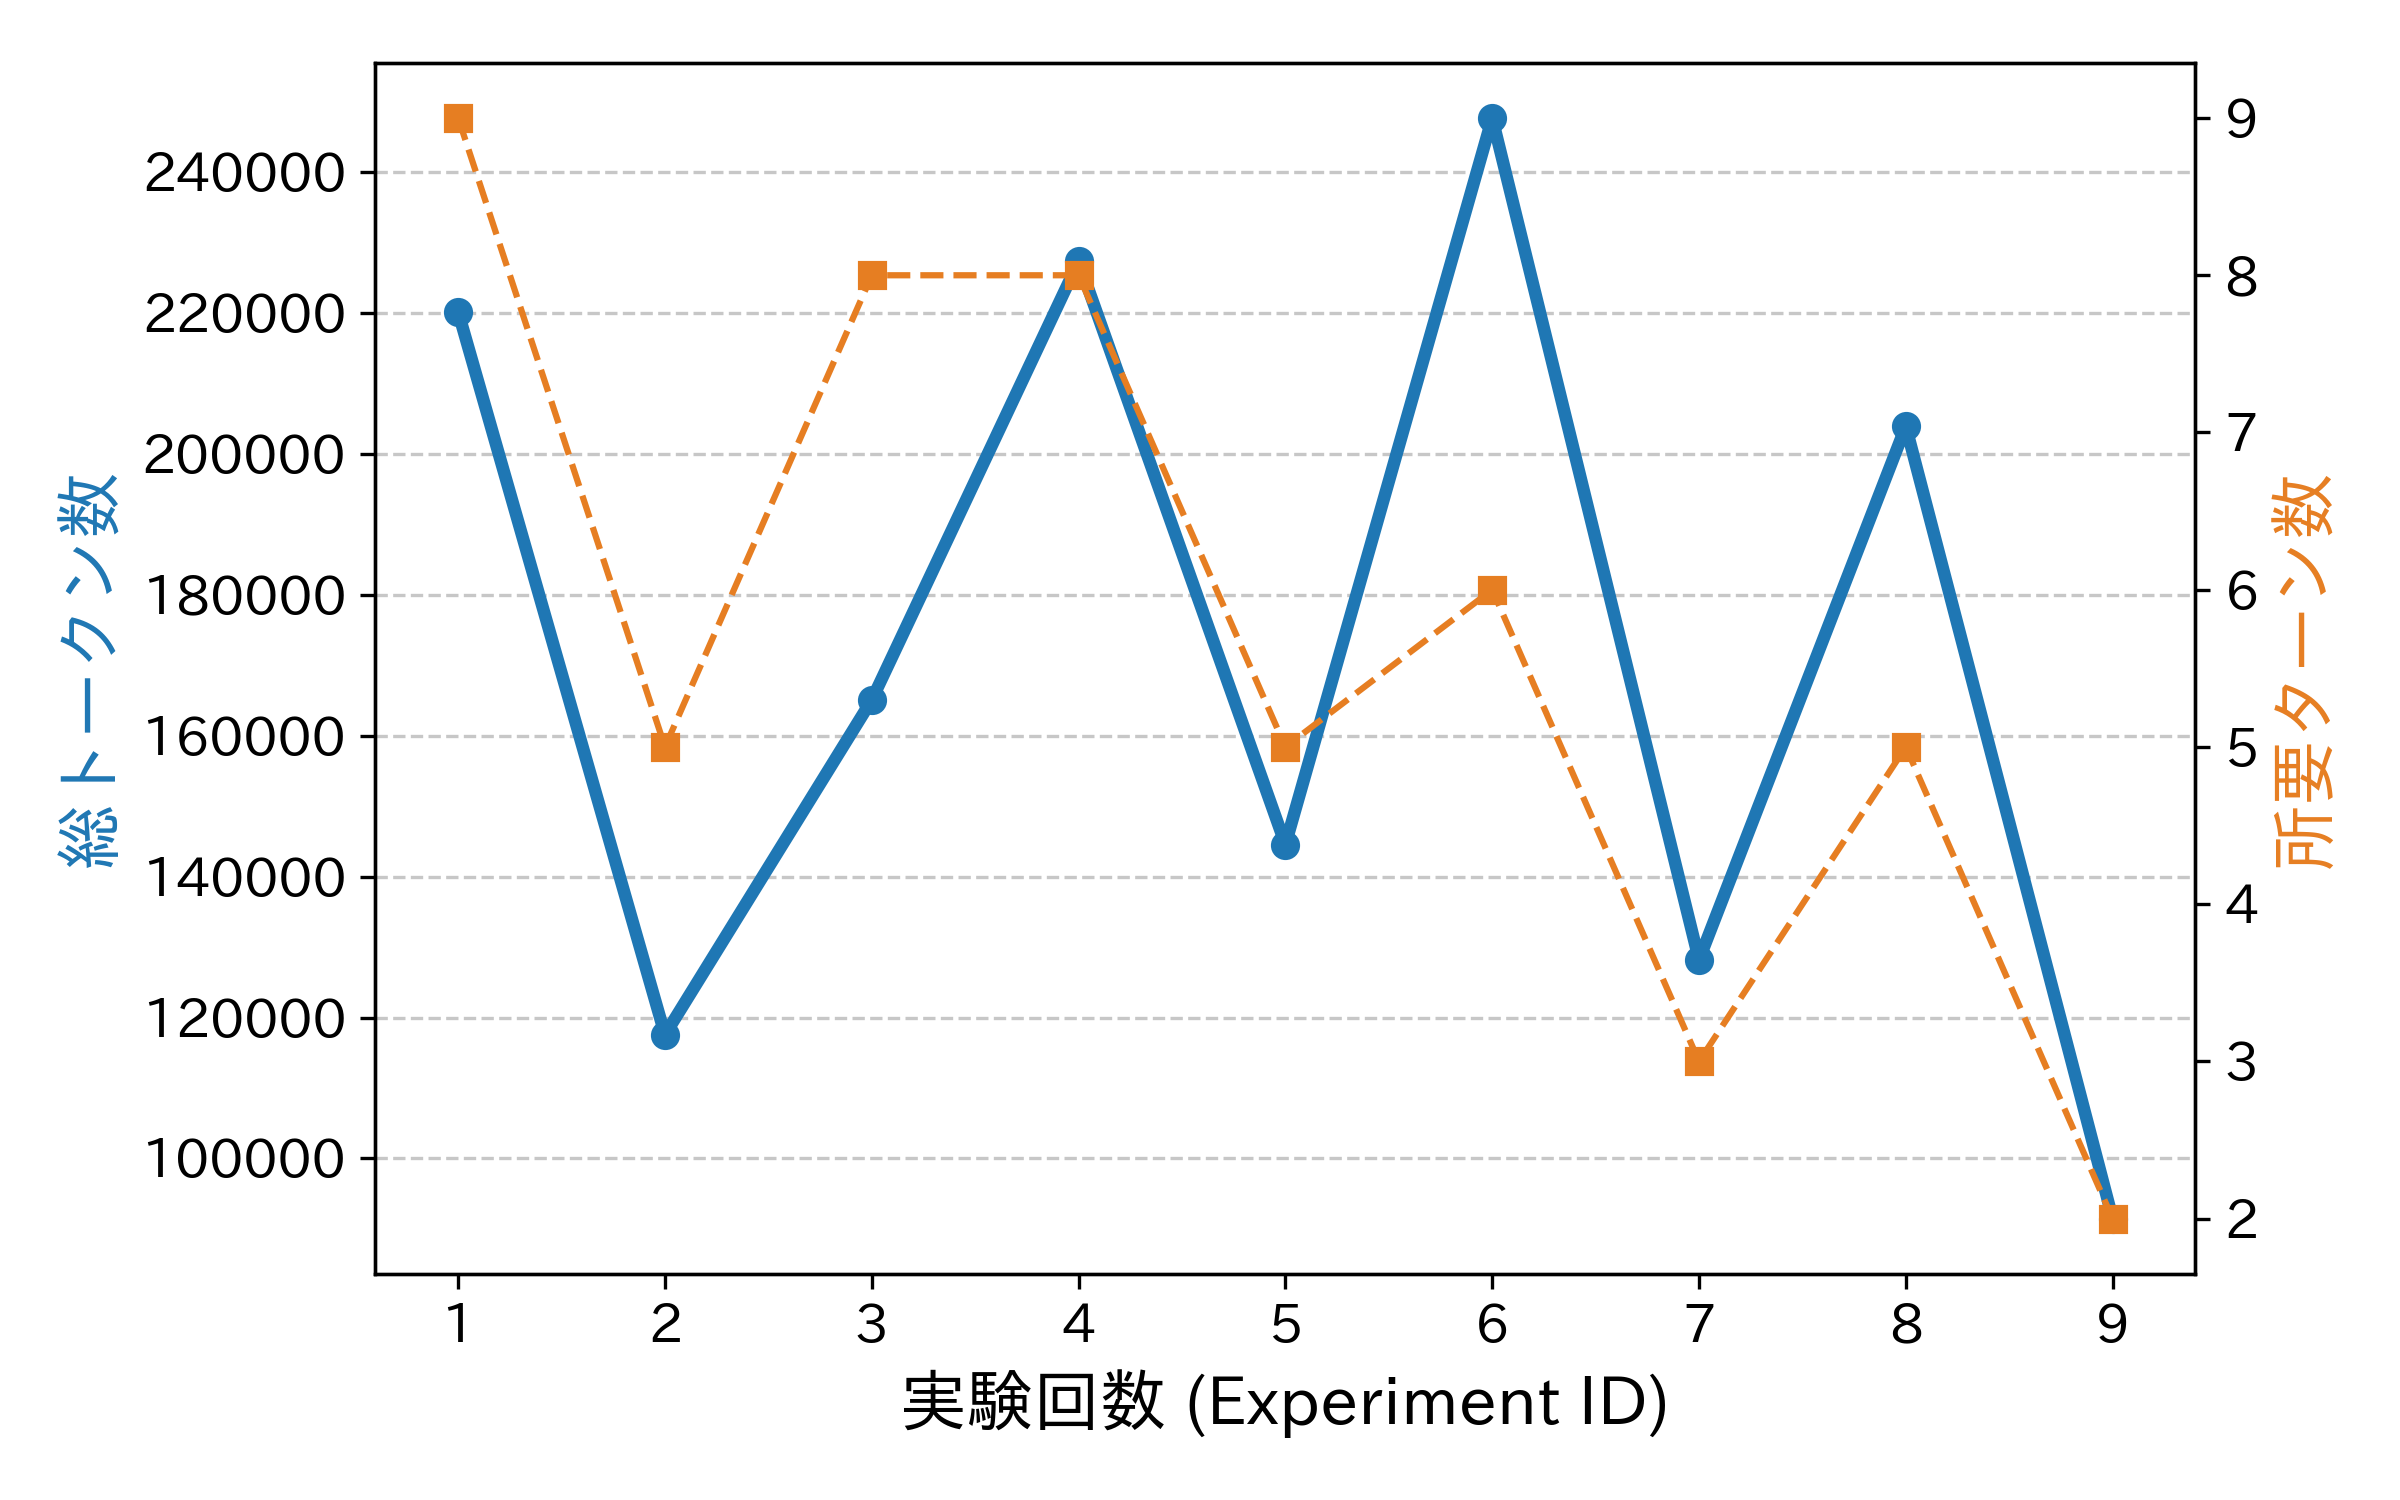
\includegraphics[width=7cm]{image/Fig3_Learning_Curve.png}
        \caption{知識蓄積に伴うコストの削減（累積トークンとターン数）}
        \label{fig:learning_curve}
    \end{center}
\end{figure}

\subsubsection{試行錯誤から即時解決への推移}

実験初期（Exp 1）の段階では，エージェントはタスク完了までに9ターンを要し，約22万トークンを消費した．実験初期の段階では，エージェントは「窓とドアの重複」や「壁高超過」といった複合的な問題に対し，ランダムなパラメータ変更と検証を繰り返す「総当たり的な探索」を行っていたことが要因である．

対照的に，知識が十分に蓄積された実験後期（Exp 9）では，わずか2ターン，約9.1万トークンで全課題をクリアしている．評価結果は初期比でターン数が約78\%削減，トークン消費量が約58\%削減されたことを意味する．ターン数とトークン消費量の削減は，エージェントが未知の探索を行わず，過去の経験則を適用するショートカットを実行したことに起因する．

\subsubsection{トークン消費の特異点と深い推論}

図\ref{fig:learning_curve}および図\ref{fig:token_cumulative}の累積トークン推移において注目すべきは，Exp 6の結果である．具体的には，6ターンに対し，全実験中で最大となる約24.8万トークンが消費されている．

Exp 6において観測されたトークン消費の増大という現象は，蓄積されたルール数（12個）が増加したことで，プロンプトに含まれるコンテキスト量が増大したこと，およびエージェントが蓄積された複数のルール間の整合性を取るために，より複雑な推論を行った結果であると解釈できる．実際にログを確認すると，Exp 6では「採光計算」と「配置制約」の競合を解消するために，Pythonコード生成と自己検証を慎重に繰り返す挙動が見られた．

しかし，Exp 6における高コストな推論は無駄ではなく，Exp 6で生成された高度な解決策がルール化されたことで，続くExp 7以降のコスト低下（Exp 7: 12.8万トークン, Exp 9: 9.1万トークン）に寄与している．推論コストの推移は，短期的コスト（投資）が長期的効率（回収）に転換されるプロセスを示唆している．

\begin{figure}[t]
 \centering
 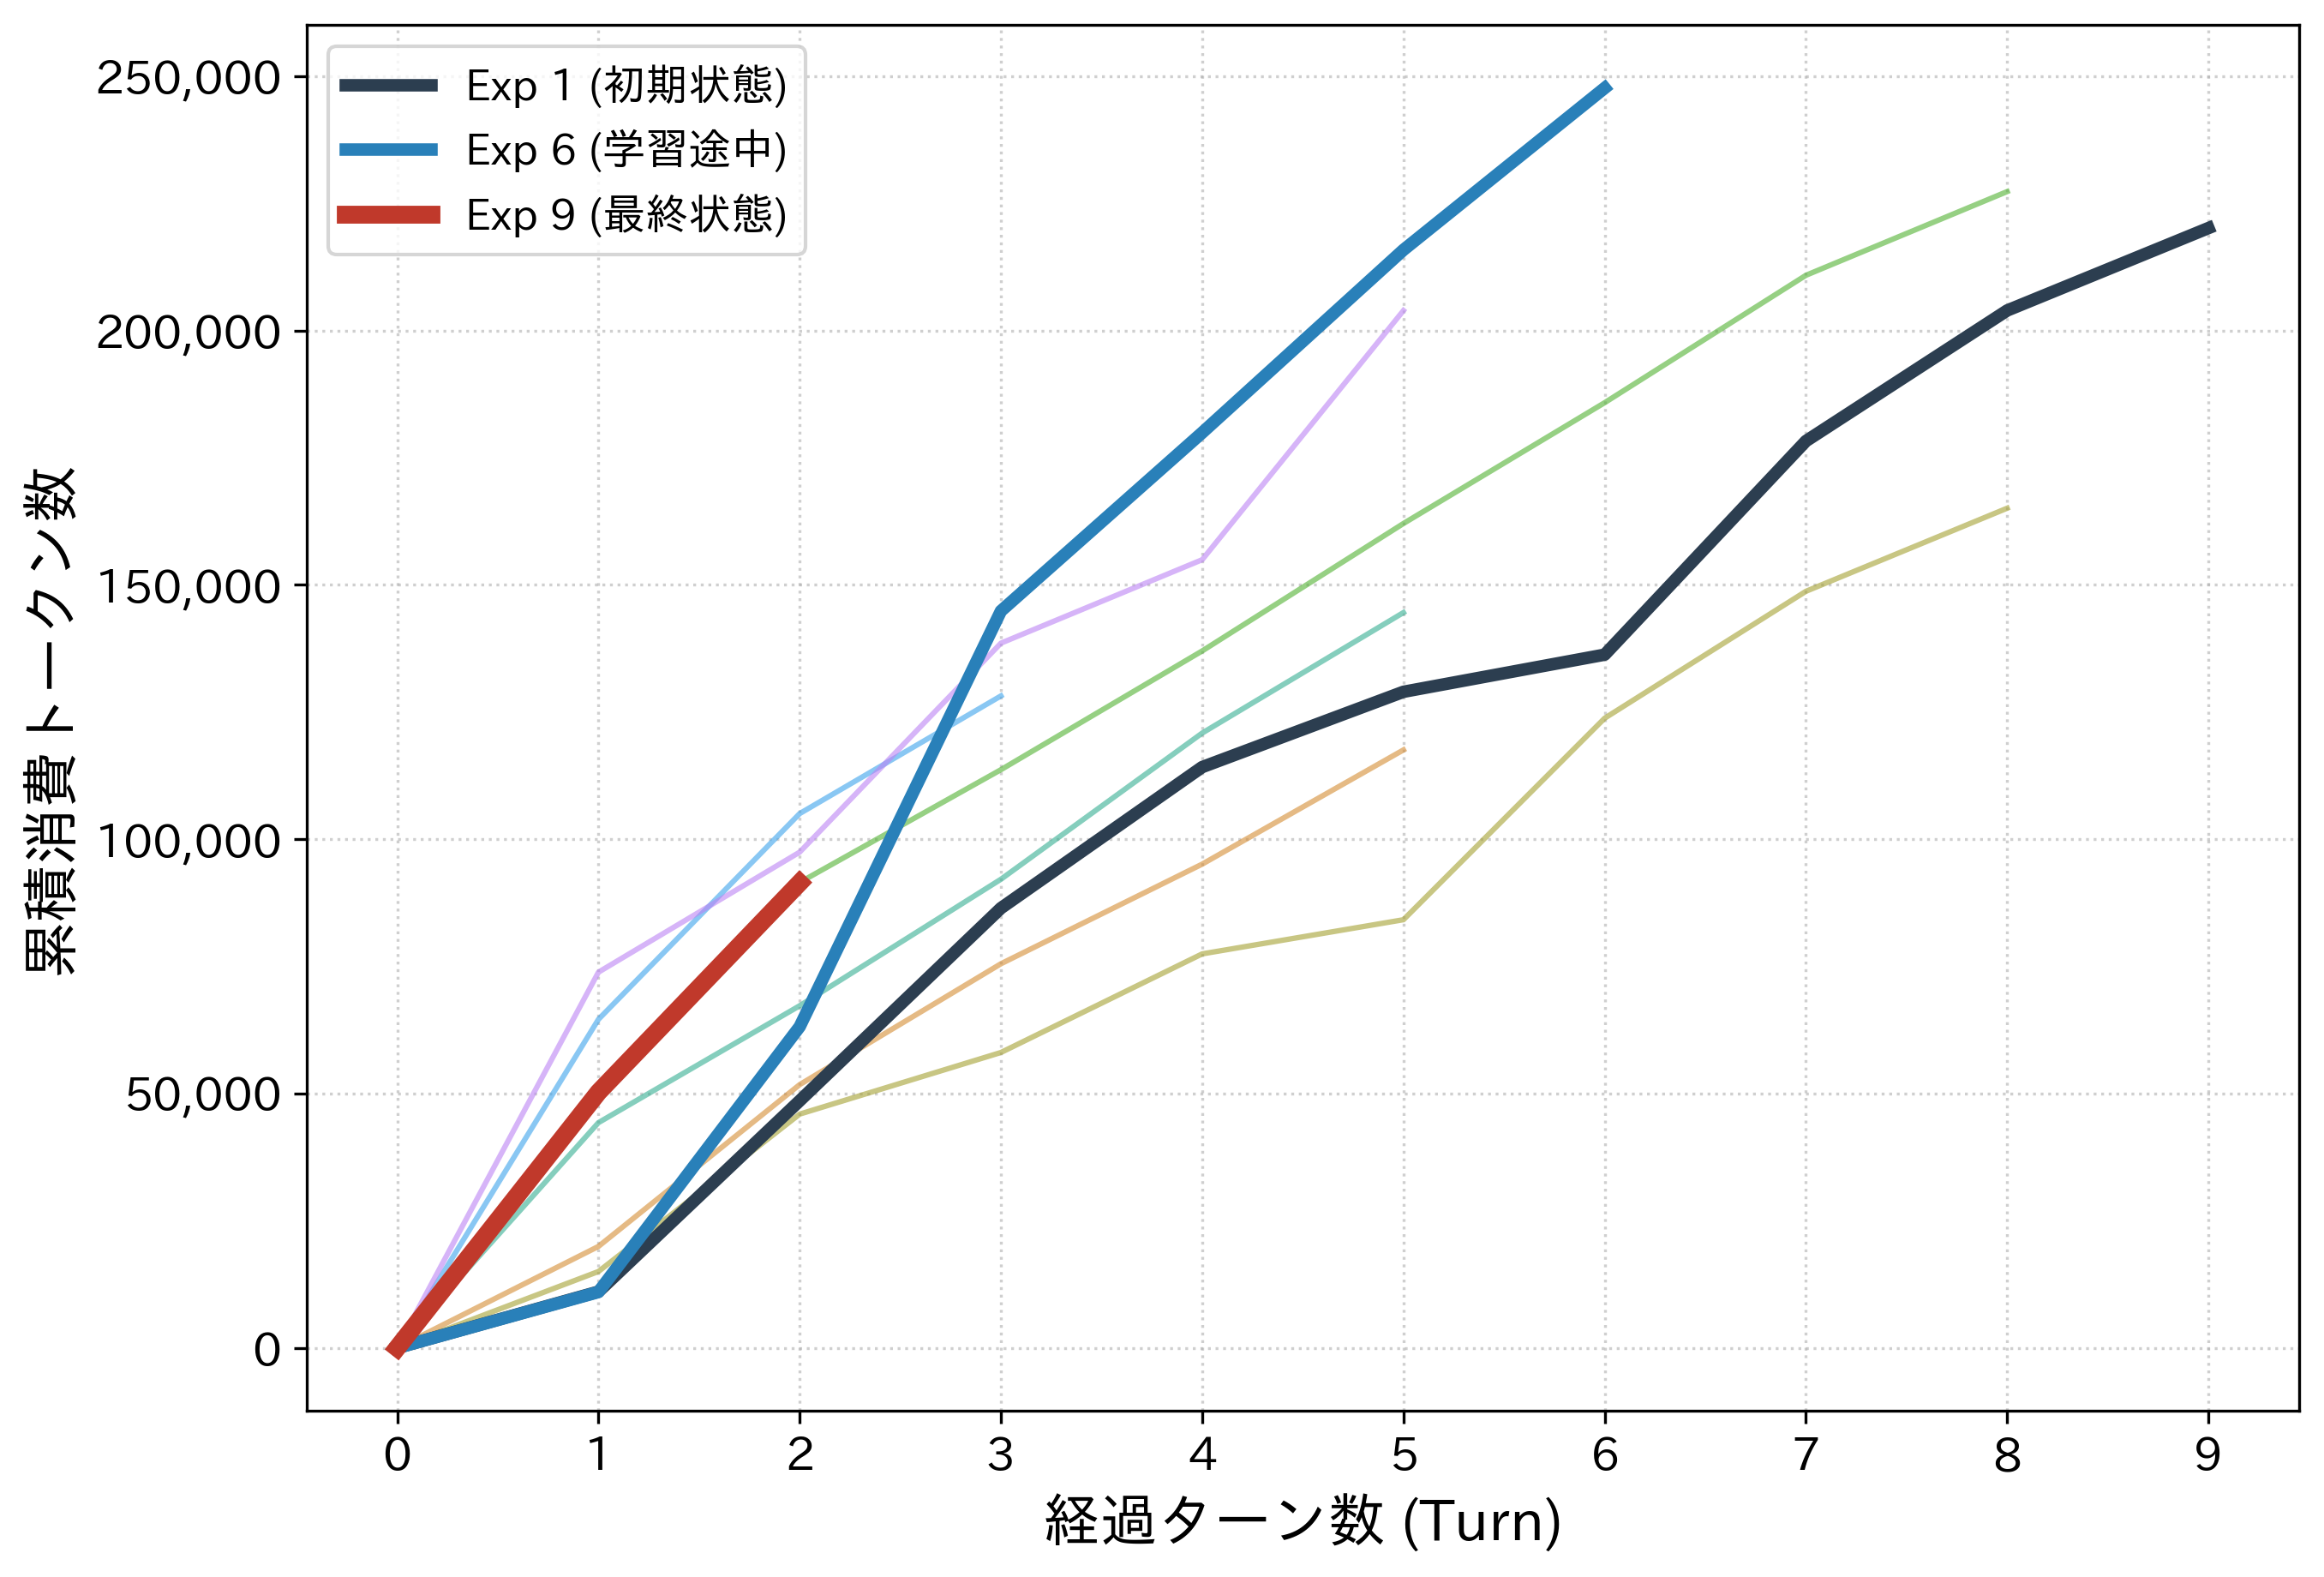
\includegraphics[width=\columnwidth]{image/Fig4_Token_Cumulative_All.png}
 \caption{セッション進行に伴う累積トークン消費の推移}
 \label{fig:token_cumulative}
\end{figure}

\subsubsection{1ターンあたりの情報密度}

図\ref{fig:token_distribution}のトークン消費分布を見ると，セッションが進むにつれて1ターンあたりの消費量は増加傾向にあることがわかる．初期は単純なAPIコールの繰り返しであったが，後期では1回の発話に「ルールの参照」や「推論」が含まれるため，1ターンあたりのトークン密度（情報量）は増加している．しかし，RAGによって試行錯誤の回数そのものが劇的に削減されるため，結果として総トークン消費量は抑制され，経済合理性が成立することが実証された．

\begin{figure}[t]
 \centering
 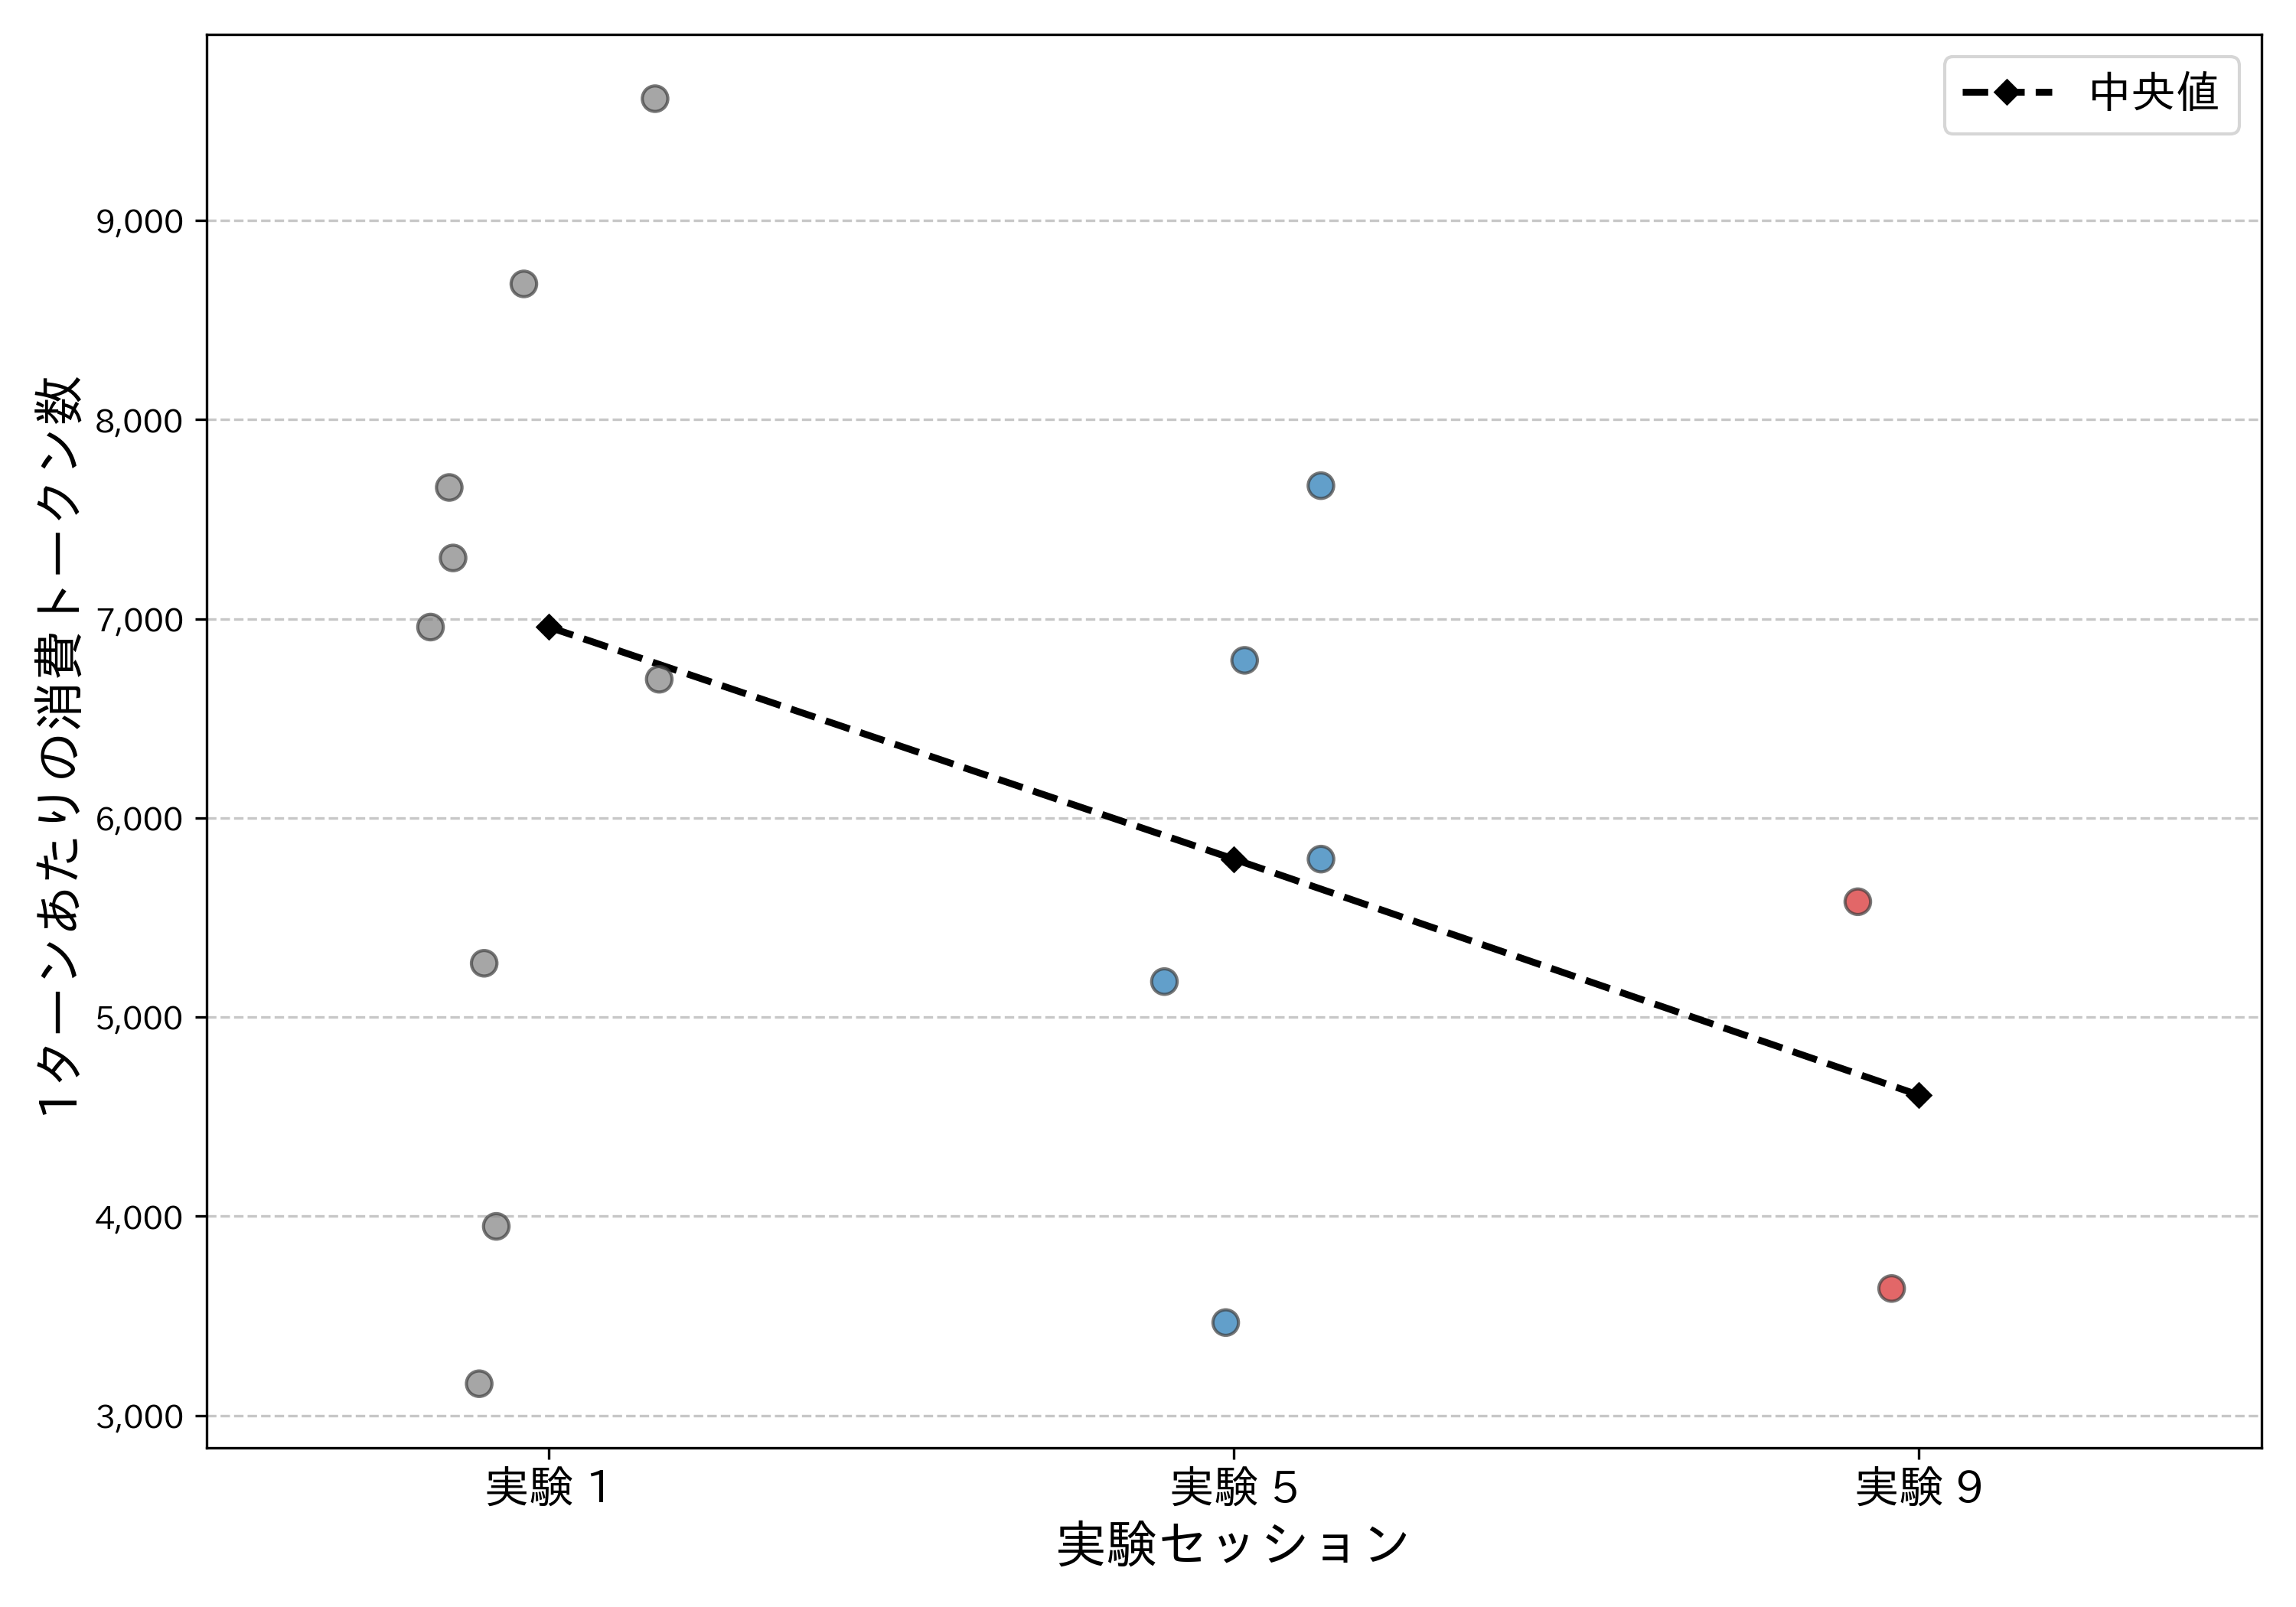
\includegraphics[width=\columnwidth]{image/Fig5_Token_Distribution_Filtered2.png}
 \caption{1ターンあたりのトークン消費量分布}
 \label{fig:token_distribution}
\end{figure}

\subsection{知識蓄積と自律性の非線形な関係}

知識が増えれば直線的に賢くなるわけではないことが，評価実験の重要な発見の一つである．図\ref{fig:knowledge_autonomy}に，累積ルール数と自律性スコアの相関を示す．

\begin{figure}[t]
 \centering
 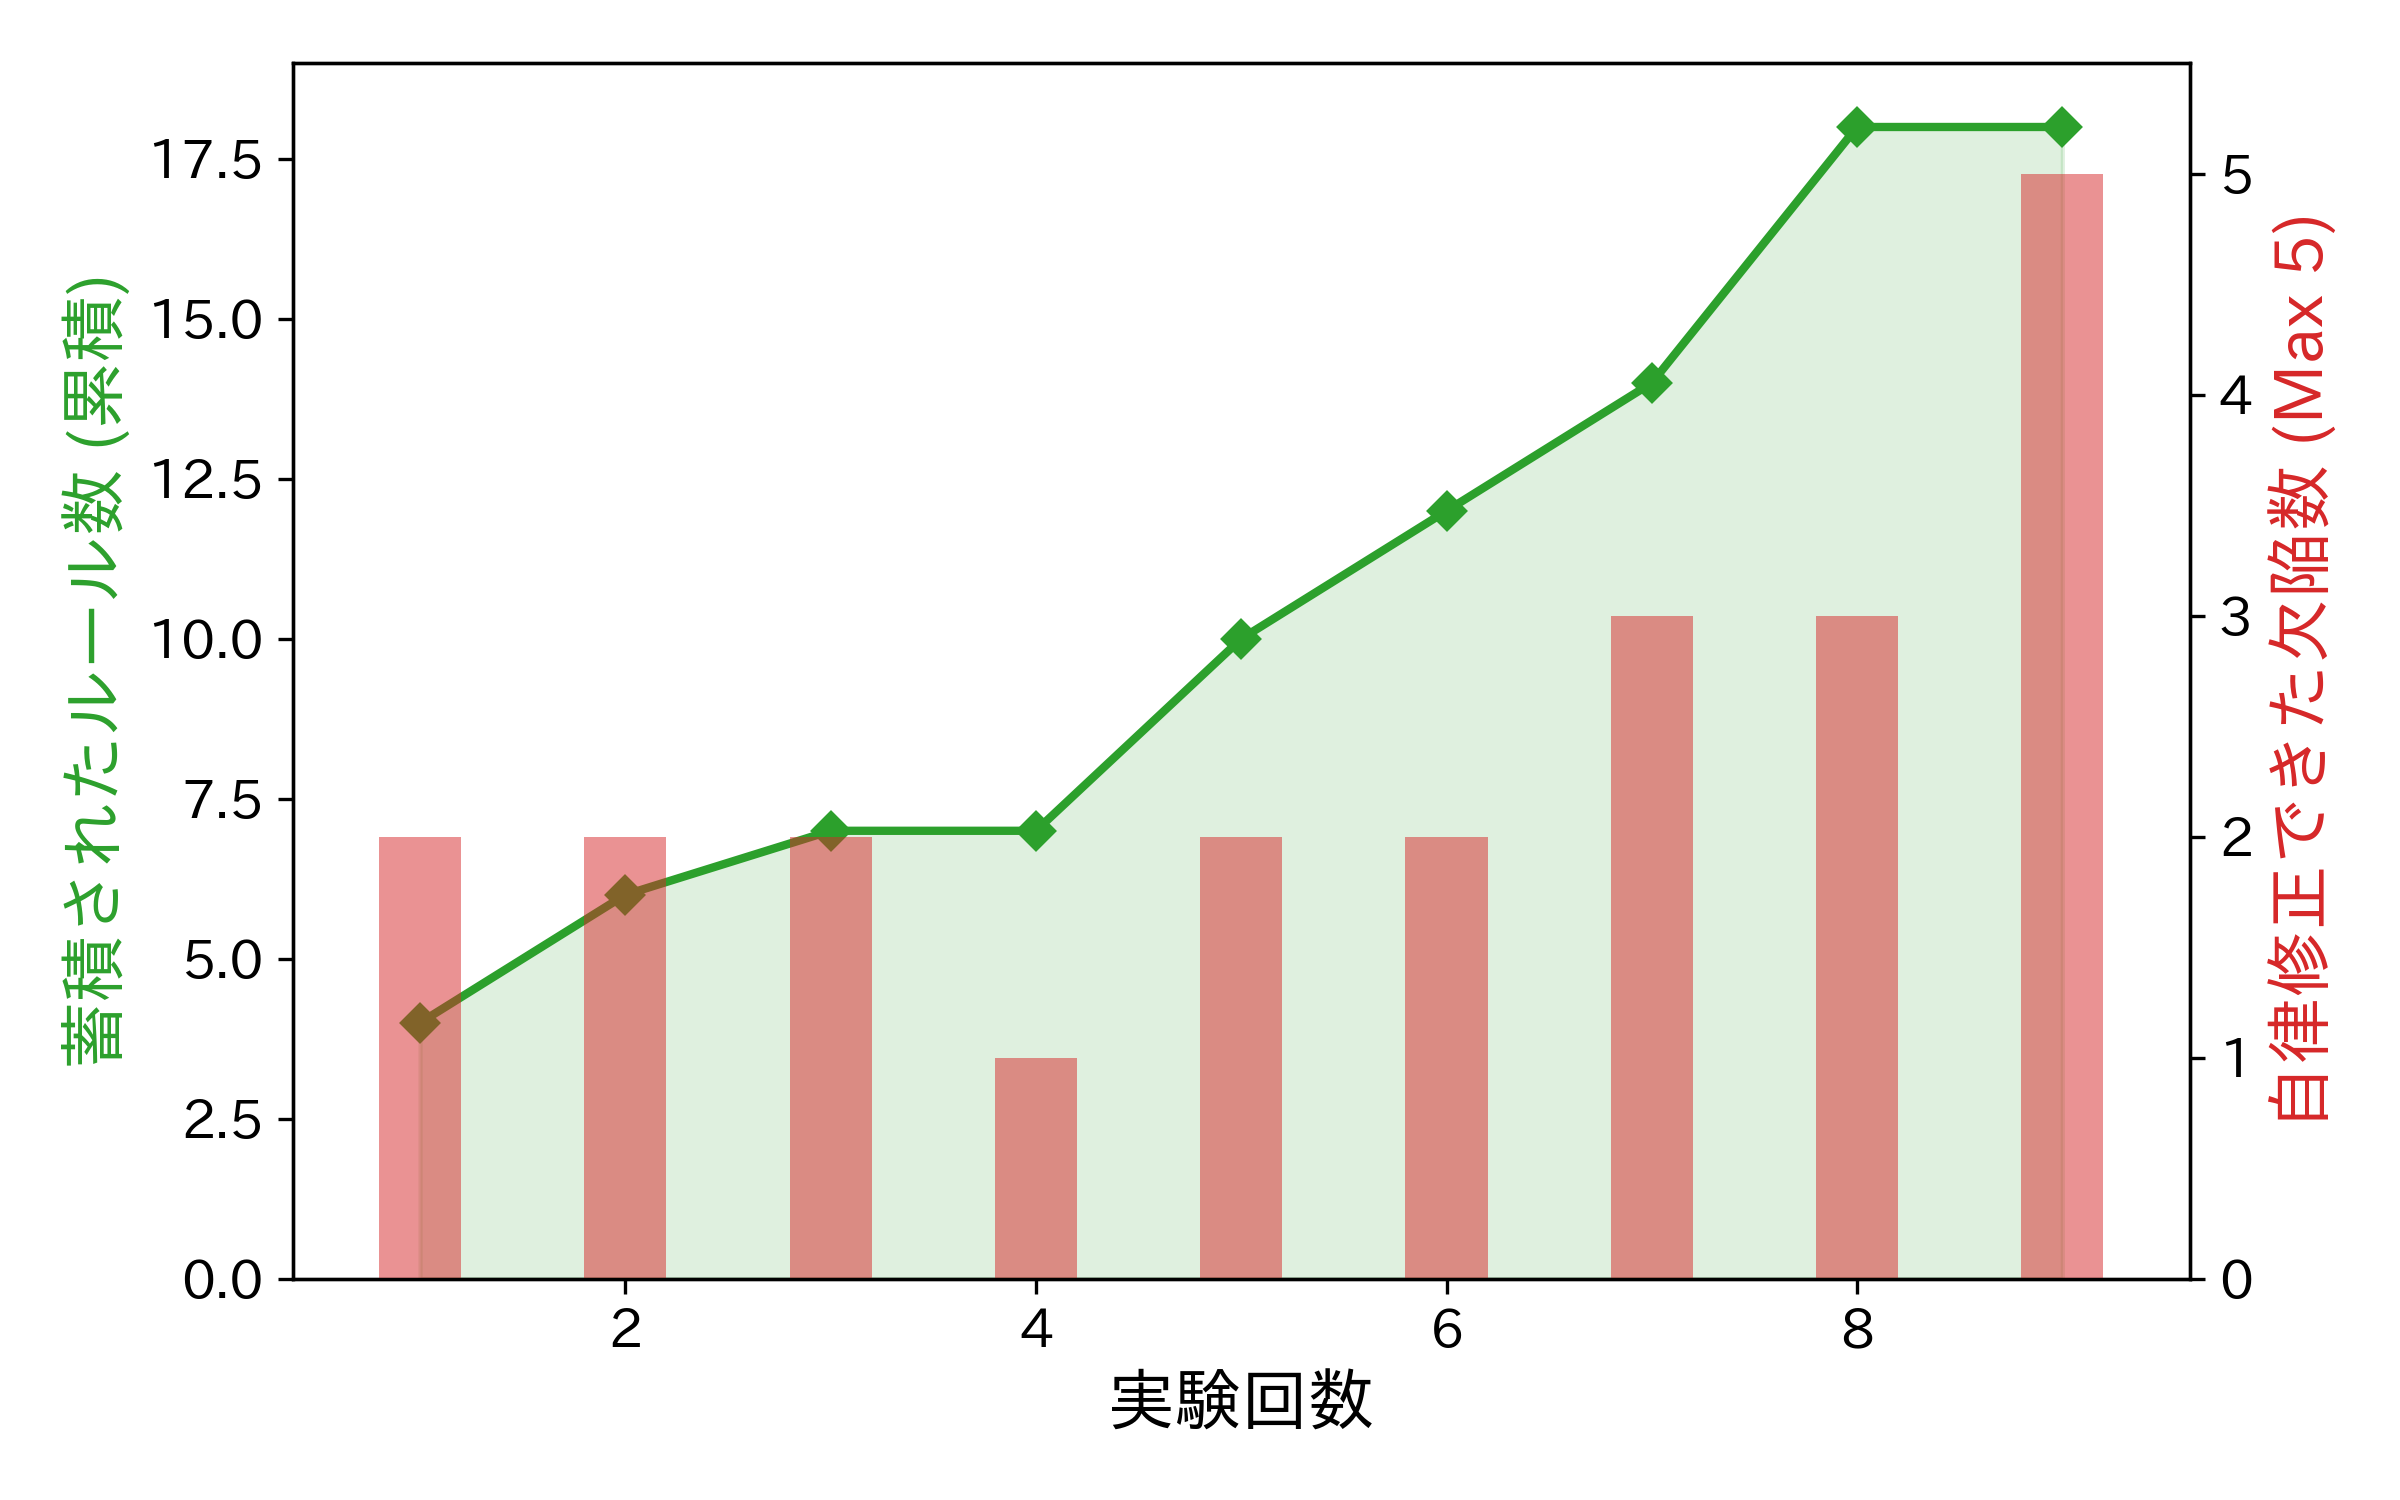
\includegraphics[width=\columnwidth]{image/Fig6_Knowledge_Autonomy.png}
 \caption{知識蓄積による自律性の向上}
 \label{fig:knowledge_autonomy}
\end{figure}

\subsubsection{知識統合に伴う一時的な停滞}

Exp 1〜3にかけて，ルール数は4から7へと順調に増加したが，自律性スコアは「2」（5つ中2つの欠陥のみ自律修正）のまま停滞した．さらにExp 4では，ルール数は7を維持しているにもかかわらず，自律性スコアが「1」（自律修正できた欠陥数が1つに減少）へと一時的に低下している．

知識蓄積に伴う自律性スコアの停滞は，認知科学における「U字型発達」\cite{strauss1982u,siegler2004u}や，システム統合時の「一時的なパフォーマンス低下」に類似している．知識ベースに断片的なルールが増えたことで，エージェントが「どのルールを優先すべきか」「どのツールを使うべきか」という判断の迷いを生じ，不適切な行動を選択する確率が高まったためと考えられる．本研究では知識蓄積に伴う自律性スコアの停滞を「知識統合に伴う一時的な停滞」と定義する．

\subsubsection{知識の体系化と完全自律への到達}

しかし，知識統合に伴う停滞は一時的なものであった．Exp 5以降，ルール数が10を超えるとスコアは回復傾向に転じ，Exp 7（ルール数14）でスコア3（3つの欠陥を自律解決），そしてExp 9（ルール数18）でついに全5つの欠陥を全て自律的に修正するスコア5に到達した．

自律性スコアの向上は，蓄積された知識がある臨界点を超えたことで，個別のルールの集合体が整合性の取れた知識ネットワークとして機能し始めたことを示している．Exp 9のエージェントは，ユーザからの曖昧な指示に対しても，「過去の採光計算ルール」や「配置クリアランスの規定」を自律的に組み合わせ，一切のヒントなしに問題を解決する能力を獲得した．

\subsection{行動変容の定性的分析：試行錯誤から熟達へ}

エージェントの「賢さ」の質的な変化は，ツール使用パターンの変容に最も顕著に表れている．図\ref{fig:tool_usage}は，初期段階（Exp 1）と熟達段階（Exp 9）におけるツール呼び出しカテゴリの比較である．

\begin{figure}[t]
 \centering
 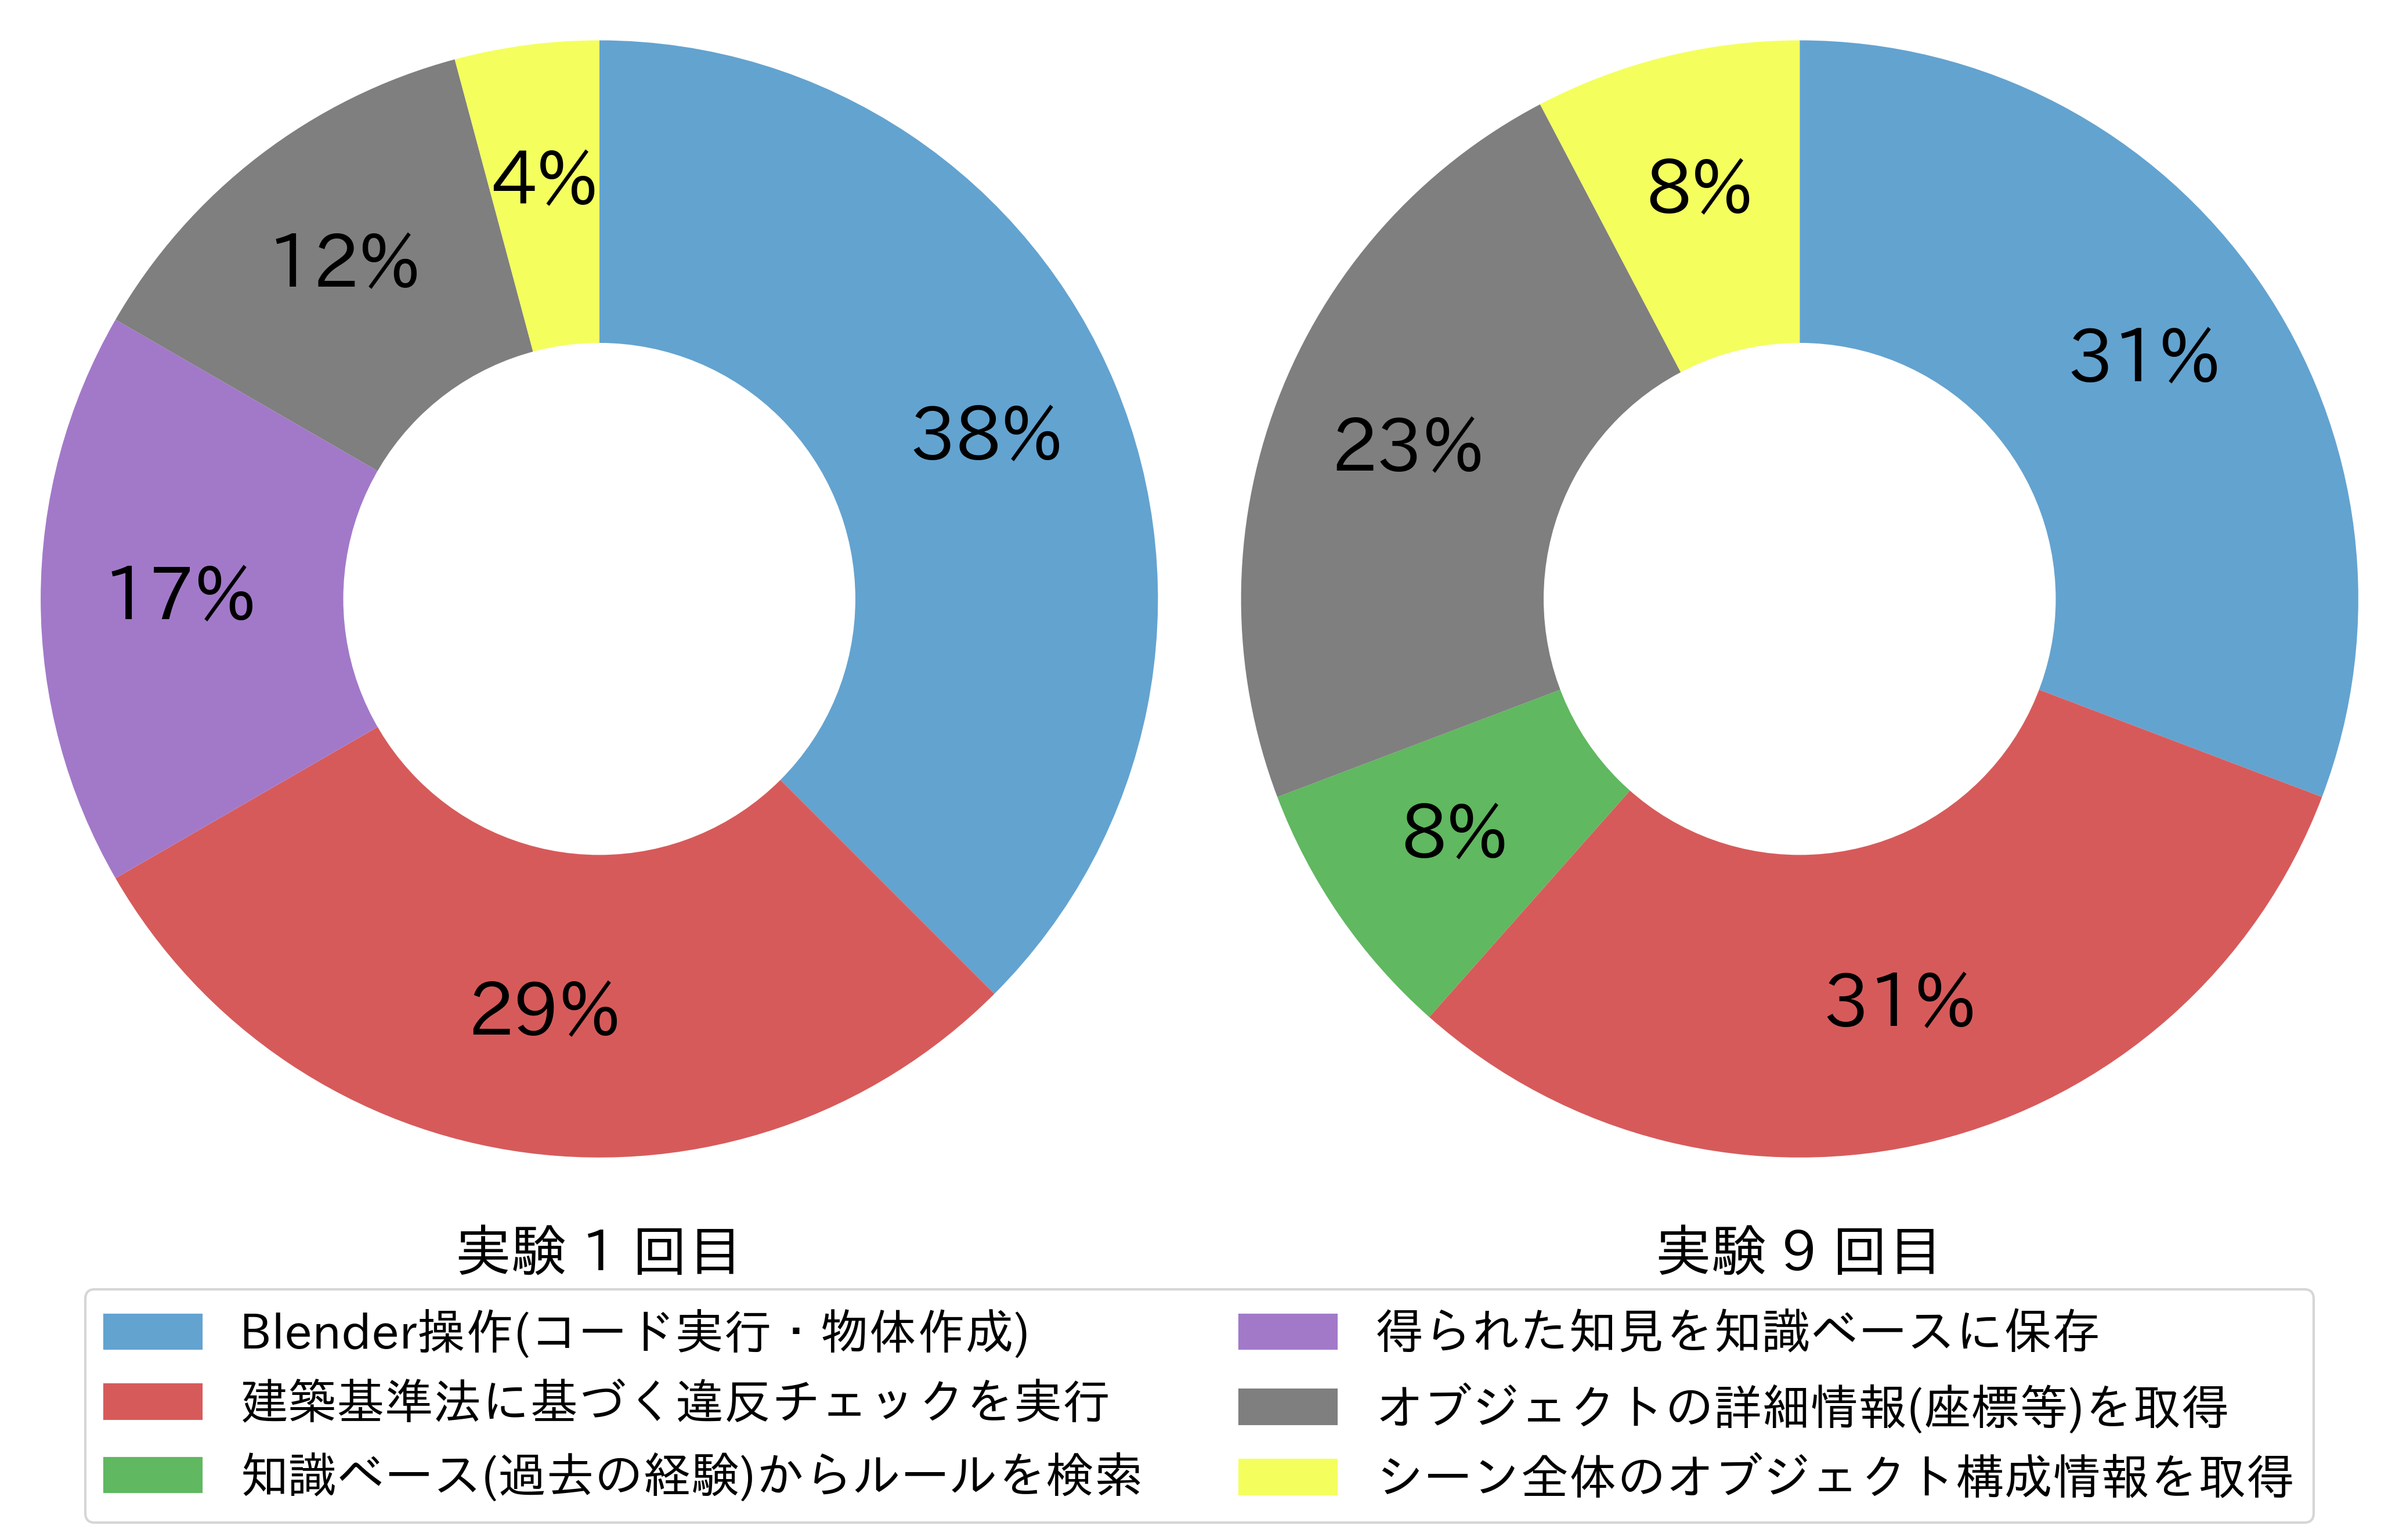
\includegraphics[width=\columnwidth]{image/Fig7_Tool_Usage.png}
 \caption{ツール使用戦略の変化（試行錯誤から知識活用へ）}
 \label{fig:tool_usage}
\end{figure}

\subsubsection{Exp 1: 試行錯誤段階}

Exp 1の行動分布（図\ref{fig:tool_usage}左）を見ると，「Blender操作」が全体の約38\%（9回），「違反チェック」が約29\%（7回）を占めている．行動分布の傾向は，操作と検証が交互に行われる「試行錯誤」のループが大半を占めていることを示している．特筆すべきは，「知見の保存」が約17\%（4回）記録されている点である．エージェントは未知の欠陥に直面するたびに解決策を獲得しており，Exp 1のフェーズではタスク遂行よりも「ルールの発見・保存」に多くのリソース（行動比重）が割かれていることが読み取れる．

\subsubsection{Exp 9: 熟達段階}

一方，Exp 9（図\ref{fig:tool_usage}右）では行動の構成比が劇的に変化している．操作と検証の比率は依然として高いものの，操作と検証の総数は激減しており，無駄なループが排除された．最も重要な変化は，「知見の保存」が消失し，代わりに「ルール検索処理」が全体の約8\%（1回）として出現している点である．わずかな比率に見えるが，知識検索へのシフトが，その後の操作精度を決定づけている．エージェントは新たにルールを獲得する（保存）のではなく，初動で過去の記憶を引き出す（検索）行動へとシフトしており，知識検索へのシフトが熟練者の行動特性である「認知の効率化」を定量的に裏付けている．

\subsubsection{具体的事例：窓とドアの重複回避}

ツール使用パターンの変容は，特に難易度の高い「窓とドアの重複（欠陥(4)）」の処理において明確であった．

\begin{itemize}
  \item \textbf{初期段階}: エージェントはまず窓を配置し，検証ツールで\texttt{Overlap Detected}というエラーを受け取ってから，少しずつ位置をずらす対処療法的な修正を行った．
  \item \textbf{後期段階}: 知識検索により「窓とドアには最低20cmのクリアランスが必要」という過去のルールを参照．配置座標を決定する段階（Pythonコード生成時）で，予めドアのバウンディングボックスを回避する計算式を組み込み，一発で干渉のない配置を実現した．
\end{itemize}

\subsection{考察}

\subsubsection{知識蓄積によるコスト削減効果}
図\ref{fig:learning_curve}に示す通り，セッションが進むにつれてトークン消費量とターン数は減少傾向にある．特に，Exp 1（初期試行）はDynamicDBに有効なルールが蓄積されていない状態であり，Exp 1の実験条件は知識継承を行わないベースライン（アブレーション条件）に相当する．
Exp 1とExp 9を比較すると，プロンプト長やモデル設定は同一であるにもかかわらず，ターン数は約78\%削減されている．ターン数とコストの差異は，RAGにより，初期のランダムなパラメータ探索が，過去の成功パターンの直接適用へと置き換わったため，試行錯誤の回数が激減したことに起因する．これは，提案する二層知識構造が推論効率の向上に直接的に寄与していることを示している．

\subsubsection{画像ベース手法に対する優位性}
SceneCraft等の既存研究は，レンダリング画像を入力とするVLMの判断に依存しているため，壁の背後にある配管の干渉や，床から1mmの浮遊といった「視覚的に認識困難な欠陥」を原理的に検出できない．
対して提案手法は，Blender内の座標データを直接参照して判定を行うため，視覚的に認識困難な欠陥であっても，本実験で設定した項目についてはすべて検出可能であった．自律性スコアがExp 9において満点（5）に達した結果は，数値的アプローチが建築のような厳密性が求められるタスクにおいて，視覚的アプローチよりも本質的に適していることを示唆している．

\subsubsection{知識統合における「停滞」のメカニズムと解消}
本実験で観測された「知識統合に伴う一時的な停滞（Exp 4）」は，エージェントが複数のルール間の競合に直面したことに起因すると考えられる．例えば，「採光面積の確保（窓を大きくする）」と「ドアとの干渉回避（窓を小さく・移動する）」という相反する制約が同時に課された際，初期の知識ベースにはそれらを調停するメタルールが存在しなかったため，エージェントは優先順位の決定に計算リソースを浪費し，結果としてパフォーマンスが低下した．

しかし，Exp 6以降の回復は，試行錯誤を通じて「干渉回避を最優先しつつ，面積要件を満たす配置を見つける」という複合的な解決戦略が新たにルール化されたことを示唆している．これは，断片的な知識が相互にリンクされ，より強固な知識ネットワークへと構造化された過程であると解釈でき，本システムが単なる知識の蓄積だけでなく，知識の洗練を行っていることを裏付けるものである．

\subsubsection{知識ベースの大規模化と検索コストの課題}
本実験ではルール数が最大18件であったため，全ルールをコンテキストに含めることが可能であったが，実運用において知識ベースが数百・数千件の規模に増大した場合，検索および推論のコストが新たな課題となる．ルール数の増加は，RAGにおける検索精度の低下や，プロンプト長の増大による応答遅延を引き起こす可能性がある．

この課題に対しては，現在の単純なキーワード・ベクトル検索に加え，タスクの文脈に応じて必要なルールのみを動的にロードする「階層的なメモリ構造」や，頻出するルールセットを統合して圧縮する「知識の蒸留」メカニズムの導入が有効であると考えられる．これらは，本システムを実社会の大規模な設計支援に応用する上で，次に取り組むべき重要な工学的課題である．

\subsubsection{数値的制約の他ドメインへの汎用性}
提案手法の核心である「数値データに基づく厳密な検査と修正」のループは，Text-to-3Dにおける建築ドメインに限定されるものではない．例えば，室内における「家具の動線確保」や，工場配管における「接続整合性の検証」，あるいは機械部品設計における「公差チェック」など，幾何学的制約として定式化可能なあらゆる生成タスクに対して適用可能である．

視覚的評価は対象の見た目やテクスチャに依存するためドメインごとの再学習が必要となる場合が多いが，本手法は「座標と寸法」という普遍的な物理量に基づいているため，検査ルールを差し替えるだけで，多様なエンジニアリングタスクへ柔軟に転用できる高い汎用性を有しているといえる．

%%%%%%%%%%%%%%%%%%%%%%%%%%%%%%%%%%%%%%%%%%%%%%%%%%%%%%%%%%%%%%%%%%%%%%%
\section{おわりに}
%%%%%%%%%%%%%%%%%%%%%%%%%%%%%%%%%%%%%%%%%%%%%%%%%%%%%%%%%%%%%%%%%%%%%%%

本研究では，3D生成における幾何学的ハルシネーションという課題に対し，MCPを用いた数値的介入と二層知識構造による解決策を提示した．提案システムは，視覚情報に依存せず，幾何データに基づく厳密な検査により，建築基準を満たすCADグレードのモデル生成を実現した．特筆すべきは，規制知識と経験知識の統合により，絶対的なルールの順守と，過去の修正事例に基づく適応的な効率化を両立させた点にある．実験データは，知識の永続化が，初期の適応停滞を乗り越え，最終的に自律性の向上と推論コストの劇的な低減に寄与することを実証した．

今後の展望として，家具配置や設備配管といったドメインへの拡張が挙げられる．これらは同様に数値的な制約充足問題として定式化可能であり，本実験では建築シーンに限定したが，家具配置や設備配管など、数値制約として定式化可能なタスク一般に適用可能である．また，現在はBlenderに限定されているMCPサーバをUnityやUnreal Engineへと展開し，より多様なシミュレーション環境での検証を進める必要がある．ただし，本実験は単一シナリオでの検証に留まっているため，より多様なタスクでの検証が必要である．加えて，実運用において知識ベースの規模が数百・数千件に増大した場合の検索コストや，ルール間の競合解消については，今後の課題である．提案手法が示した「数値的リアリズム」の追求と知識継承モデルは，生成AIを単なるクリエイティブツールから，信頼性が不可欠なエンジニアリングや製造の現場で活用可能な自律システムへと昇華させるための重要な基盤となるであろう．

%%%%%%%%%%%%%%%%%%%%%%%%%%%%%%%%%%%%%%%%%%%%%%%%%%%%%%%%%%%%%%%%%%%%%%%
% 参考文献
%%%%%%%%%%%%%%%%%%%%%%%%%%%%%%%%%%%%%%%%%%%%%%%%%%%%%%%%%%%%%%%%%%%%%%%

\bibliographystyle{junsrt}
\bibliography{reference}

\end{document}